\documentclass[10pt,twocolumn]{article}

\usepackage[margin=0.75in]{geometry}
\usepackage{amsmath,amssymb,amsthm}
\usepackage{booktabs,multirow,array,longtable}
\usepackage{graphicx}
\usepackage{float}
\usepackage{enumitem}
\usepackage{hyperref}
\usepackage{setspace}
\usepackage{xcolor}
\usepackage{natbib}
\usepackage{caption}
\usepackage{subcaption}

\setlength{\columnsep}{0.25in}
\setlength{\parskip}{0.3em}
\setlength{\parindent}{0em}

\title{A Probabilistic Risk Assessment and Risk-Averse Optimization Framework for Sewer Spill Reduction in Wastewater Utilities}

\author{Ramesh Manian, Khang Do, Annabelle Jayadinata, Maura Osorio \\ Sponsor: Chris Foley \\ Stanford University}

\date{}

\begin{document}

\maketitle

\begin{abstract}
This paper develops a probabilistic risk assessment (PRA) and risk-averse
optimization framework for sanitary sewer spill mitigation in wastewater
utilities. The framework integrates historical spill data, severity-category
modeling, spill-volume modeling, probabilistic spill occurrence estimation,
and operational priors for sparse failure modes. Risk-averse investment
allocation is achieved through expected utility maximization with an
exponential utility function calibrated to the utility's risk tolerance,
combined with Monte Carlo simulation over stochastic spill outcomes. A case
study using 26 years of spill history from the Carmel Area Wastewater
District (CAWD) demonstrates how the framework converts operations and
maintenance investment decisions into quantified spill-risk reduction
outcomes, including reductions in expected annual spill cost and
high-severity tail exposure.
\end{abstract}
 
% --- PASTE THIS AS SECTION 1 ---
 
\section{Introduction}
 
\subsection{Motivation}
 
Aging wastewater infrastructure, increasing regulatory scrutiny,
climate-driven hydraulic stress, and constrained operational budgets have
elevated the importance of quantitative risk-informed decision making in
wastewater utilities. Sanitary sewer overflows (SSOs) are unintended
releases of untreated wastewater from collection systems prior to reaching
a treatment facility. The consequences of SSOs range from localized
property damage to large-scale surface-water contamination, beach closures,
and regulatory enforcement actions---and they are fundamentally preventable
through targeted operations and maintenance (O\&M) investment.
 
The Carmel Area Wastewater District (CAWD) operates approximately 81 miles
of gravity and force-main sewer infrastructure serving roughly
11{,}000 residents on California's central coast. Wastewater collected
from the service area travels by gravity to a wet well, is pumped through
headworks for screening and grit removal, and then proceeds through primary
clarification, biological treatment, and tertiary microfiltration and
reverse osmosis before reclaimed water is delivered to Pebble Beach golf
courses. Any failure in the collection network prior to the headworks
constitutes an SSO: untreated wastewater releases directly to the
environment without any treatment barrier. This makes collection system
integrity the first and most consequential line of defense in CAWD's
environmental protection strategy.
 
CAWD's environmental exposure from SSOs is amplified by its geography.
The collection system discharges to a treatment plant situated adjacent to
the Carmel River lagoon, a coastal water body subject to active hazard
monitoring under a Coastal Development Permit from the California Coastal
Commission \citep{cawd_hazards2025}. The district's service area is further
bounded by Carmel Bay, designated as an Area of Special Biological
Significance under California's Ocean Plan. Any Category~1 spill that
reaches a drainage channel, the river, or the bay carries disproportionate
environmental and regulatory consequences relative to a contained spill of
the same volume. This geographic reality motivates the severity-weighted
cost structure at the core of the framework developed in this paper.
 
Despite these risk-amplifying conditions, CAWD faces a spill rate higher
than comparable utilities and currently lacks a quantitative framework
connecting O\&M investment decisions to spill-risk reduction outcomes. The
district seeks a data-driven plan to minimize the cost of spill
consequences under a fixed O\&M budget. This paper addresses that objective
through three integrated components:
 
\begin{enumerate}[leftmargin=*]
    \item A \textbf{failure-mode probabilistic risk model} that decomposes
    annual spill risk into five mutually exclusive failure modes (blockage,
    pipe failure, pump failure, hydraulic overload, and operational failure),
    each modeled as a Poisson process with rate calibrated from 26 years of
    CAWD historical spill records.
 
    \item A \textbf{Risk Averse Optimization} that allocates CAWD's
    annual O\&M budget across four investment levers to maximize expected utility. It allocates to the candidate with the lowest negative expected utility objective. 
\end{enumerate}
 
The consequences of deferred maintenance on aging sewer infrastructure are
neither abstract nor distant. In January 2026, a sewer collapse released an
estimated 240 to 300 million gallons of untreated sewage into the Potomac
River, one of the largest such spills in U.S. history. In April 2026, a
federal judge found Mountain View, California in violation of the Clean
Water Act and imposed nearly \$1.2 million in civil penalties for allowing
raw sewage to enter Stevens Creek. Both cases illustrate the same failure:
deferred maintenance on aging infrastructure produces environmental damage,
regulatory liability, and remediation costs that dwarf the cost of
proactive risk management. For a utility like CAWD, situated adjacent to
environmentally sensitive coastal waters, the asymmetry between prevention
cost and consequence cost is particularly stark.
 
\subsection{Research Gap}
 
Despite substantial progress in both wastewater asset management and
probabilistic risk analysis, existing approaches rarely combine these
methods into a single decision-support framework usable by small- and
mid-sized utilities. In particular, the literature exhibits the following
gaps:
 
\begin{itemize}[leftmargin=*]
    \item \textbf{Lack of integrated probabilistic risk assessment (PRA)
    for sewer systems.} Most utility risk studies focus on individual
    failure modes in isolation rather than decomposing total spill risk
    into a coherent set of mutually exclusive, exhaustive failure modes
    with associated occurrence rates, severity distributions, and cost
    consequences \citep{johnson2021}.
 
    \item \textbf{Absence of severity-weighted spill modeling.} Existing
    benchmarking practices typically report raw spill counts or volumes
    without weighting by regulatory category or environmental consequence,
    which obscures the disproportionate contribution of Category~1
    surface-water discharges to total risk.
 
    \item \textbf{No explicit treatment of catastrophic spill events.}
    Sanitary sewer overflows exhibit heavy-tailed cost distributions, yet
    most utility planning tools rely on expected-value criteria or
    deterministic schedules that systematically underweight rare,
    high-consequence events.
 
    \item \textbf{Minimal utility-theoretic framing of public
    infrastructure risk.} Wastewater utilities operate under
    multi-objective constraints (regulatory compliance, environmental
    stewardship, public trust, fiscal accountability) that warrant
    explicit decision-analytic treatment, yet most operational planning
    tools remain deterministic \citep{halfawy2008}.
\end{itemize}
 
This study addresses these gaps by integrating failure-mode-specific PRA,
severity-weighted spill modeling, Monte Carlo simulation, and
expected-utility-based risk-averse optimization within a single
decision-support framework calibrated to a real wastewater utility.
 
\subsection{Contributions}
 
This paper makes the following contributions:
 
\begin{enumerate}[leftmargin=*]
    \item \textbf{A normalized probabilistic spill-risk framework} that
    decomposes annual SSO risk into five mutually exclusive failure modes
    (blockage, pipe failure, pump failure, hydraulic overload, operational
    failure) and expresses each as a Poisson process with rate calibrated
    from historical utility data.
 
    \item \textbf{Failure-mode-specific spill modeling} that links
    operational and maintenance investments to mode-level spill rates
    through an exponential effectiveness function, capturing diminishing
    returns on O\&M spending.
 
    \item \textbf{Severity-category and spill-volume modeling} that
    translates spill occurrence into regulatory category and discharge
    volume distributions, enabling explicit modeling of Category~1
    surface-water impacts and their disproportionate cost consequences.
 
    \item \textbf{Integration of O\&M investments with spill-risk
    reduction} via a Lagrangian convex optimization that allocates a
    constrained budget across four investment levers (preventive
    maintenance, workforce capacity, execution reliability, risk-based
    targeting) to minimize expected annual spill cost.
 
    \item \textbf{Risk-averse optimization under catastrophic spill
    exposure} using a Monte Carlo--expected utility formulation with
exponential utility $U(-C) = 1 - e^{C/\rho}$, calibrated to CAWD's
risk tolerance $\rho = \$10$M, which penalizes high-cost tail
outcomes beyond what expected value alone captures.
 
    \item \textbf{A real wastewater utility case study} demonstrating
    the framework using 26 years of spill history from CAWD, with
    results showing reduction in both expected annual spill cost and
    high-severity tail exposure under the optimized investment policy.
\end{enumerate}
 
\section{Background and Literature Review}
 
\subsection{Wastewater Spill Risk and Utility Management}


Sanitary sewer overflows (SSOs) are unintended releases of untreated
wastewater from collection systems prior to reaching a treatment facility.
The U.S.\ Environmental Protection Agency estimates that between
23{,}000 and 75{,}000 SSO events occur annually in the United States
\citep{epa2024}, with consequences ranging from localized property damage
to large-scale surface-water contamination, beach closures, and regulatory
enforcement actions. In California, SSOs are regulated under the State
Water Resources Control Board (SWRCB) Statewide General Order, which
establishes mandatory reporting requirements and four spill severity
categories based on volume, recovery, and surface-water impact. For
utilities operating adjacent to designated sensitive receiving waters---such
as areas of special biological significance or actively monitored coastal
lagoons---the consequence differential between Category~1 surface-water
discharges and lower-category contained spills is particularly pronounced,
further motivating the severity-weighted risk framework developed in this
paper.
 
Structural and operational failures in sewer systems are inherently
multifactorial. \citet{davies2001} identify three primary causal domains:
construction-related factors (material selection, joint integrity,
installation quality), external factors (soil movement, root intrusion,
traffic loading), and operational factors (flow velocity, debris
accumulation, hydraulic overload). \citet{scheidegger2015} unify nine
families of deterioration models under a common ``bathtub-with-jumps''
hazard framework and emphasize the importance of treating right-censoring
and survival selection bias when calibrating failure models from historical
inspection data. \citet{duchesne2013} extend this perspective through
survival analysis with explicit likelihood functions for censored
observations.
 
For mid-sized utilities, \citet{foreroortiz2023} review 103 publications
on sewer failure prediction and conclude that explanatory variables
(previous failures, segment length, material, age) exert greater predictive
influence than algorithmic choice, and that severe class imbalance (failure
rates near 0.1\%) complicates direct application of standard classifiers.
This finding motivates the operational-prior approach adopted in the present
study for sparse failure modes.
 
The primary physical failure mechanisms observed in the CAWD collection
system are summarized in Table~\ref{tab:failure-mechanisms}, together with
their dominant drivers, standard mitigation strategies, and the baseline
spill rates $\lambda_{k0}$ (in spills per 100 miles per year) calibrated
from the 26-year historical record. Blockage dominates both in frequency
and in total system risk, driven by root intrusion into aging vitrified
clay pipe (VCP). Pipe failure ranks second in baseline rate and carries
a higher expected cost per spill due to its elevated probability of
surface-water impact. The three remaining failure modes---pump failure,
hydraulic overload, and operational failure---are sparse in the historical
record and are assigned rates informed by operational priors, as described
in Section~5.2.
 
\begin{table*}[t]
\centering
\caption{Primary Failure Mechanisms, CAWD Historical Prevalence, and
         Baseline Spill Rates (2000--2026)}
\label{tab:failure-mechanisms}
\begin{tabular}{p{2.2cm} p{3.0cm} p{3.5cm} p{2.0cm} p{2.0cm}}
\toprule
\textbf{Failure Mode} & \textbf{Primary Driver} & \textbf{Mitigation Strategy}
  & \textbf{CAWD Status} & \textbf{$\lambda_{k0}$\textsuperscript{a}} \\
\midrule
Blockage
  & VCP joints; root intrusion; FOG
  & Chemical treatment; hydro-jetting; CCTV inspection
  & Dominant
  & 6.48 \\[4pt]
Pipe Failure
  & Material aging; soil movement
  & CIPP lining; pipe bursting; targeted replacement
  & High
  & 0.88 \\[4pt]
Pump Failure
  & Mechanical/electrical wear
  & Redundancy; SCADA monitoring
  & Moderate
  & 0.049\textsuperscript{b} \\[4pt]
Hydraulic Overload
  & Inflow \& Infiltration (I\&I)
  & Smoke testing; manhole sealing
  & Low (Data Gap)
  & 0.20\textsuperscript{b} \\[4pt]
Operational Failure
  & Human error; procedure gaps
  & Training; standard operating procedures
  & Rare
  & 0.10\textsuperscript{b} \\
\bottomrule
\end{tabular}
\smallskip
 
\noindent\footnotesize
\textsuperscript{a}~Spills per 100 miles per year, calibrated from the
2000--2026 CAWD spill tracking record (system length 77.57 miles used
for normalization; see Section~5.1).\\
\textsuperscript{b}~Rate informed by operational prior due to sparse
historical observations; see Section~5.2.
\end{table*}
 
As shown in Table~\ref{tab:failure-mechanisms}, \textbf{root intrusion}
is the dominant failure mode in the CAWD system, reflecting the prevalence
of older VCP segments with permeable joints in proximity to mature trees.
Root masses penetrate joint seals, restrict flow, and accumulate debris,
producing the high-frequency blockage events that drive annual spill counts.
\textbf{Structural pipe failure} ranks second in prevalence and arises from
material aging, soil movement, and external loading; rehabilitation via
CIPP lining and targeted replacement is the standard mitigation.
\textbf{Fats, oils, and grease (FOG) and debris accumulation} are captured
within the blockage mode and driven by upstream commercial and residential
discharges, mitigated through FOG inspections and public education.
\textbf{Pump station failures} occur at moderate frequency and are addressed
through mechanical redundancy and SCADA-based condition monitoring.
\textbf{Hydraulic overload} from inflow and infiltration (I\&I) is reported
at low frequency in CAWD records, but this likely reflects a data-coding
gap rather than true rarity; \citet{brandstetter1996} document up to 88\%
RDI\&I reduction following targeted rehabilitation, suggesting hydraulic
overload warrants explicit modeling even when underreported. This data gap
motivates the operational-prior treatment adopted in Section~5.2.
 
\subsection{Probabilistic Risk Assessment (PRA)}
 
Probabilistic risk assessment (PRA) originated in the nuclear power
industry and provides the methodological foundation for this study.
\citet{kaplan1981} established the canonical quantitative definition of
risk as a set of triplets $\langle S_i, P_i, X_i \rangle$, where $S_i$
is a scenario, $P_i$ is its probability, and $X_i$ is its consequence.
This triplet structure---scenario identification, probability estimation,
and consequence quantification---maps directly onto the failure-mode
decomposition developed in this paper: each failure mode $k$ constitutes
a scenario class, its Poisson rate $\lambda_k$ characterizes its
probability, and the severity-weighted cost $W_k$ quantifies its
consequence.
 
PRA has since been extended to civil infrastructure systems, including
water and wastewater networks. \citet{johnson2021} demonstrate the
feasibility of applying the PRA framework to networked infrastructure,
noting that while PRA is standard practice in nuclear and industrial safety
settings, it has not been widely adopted for water and sewer systems despite
the analytic tools being directly transferable. Their central finding is
that the primary barrier is not methodological but operational:
infrastructure analyses routinely omit the likelihood-assessment component
of PRA, treating failures as deterministic rather than probabilistic events.
The present study addresses this gap directly by calibrating failure-mode
Poisson rates from 26 years of CAWD historical spill records and embedding
them in a full probabilistic consequence model.
 
For high-frequency, low-individual-consequence events such as sewer
blockages, the Poisson process is the standard occurrence model for
pipeline failure frequency estimation \citep{dawotola2013}. Each failure
mode $k$ is characterized by an annual rate $\lambda_k$, and observed
spill counts $n_k$ over an observation horizon $T$ yield
maximum-likelihood estimates $\hat{\lambda}_k = n_k / T$. For failure
modes where $n_k$ is small or zero, direct maximum-likelihood estimation
produces degenerate zero-rate estimates that understate true system risk.
Bayesian inference with operationally informed priors avoids this problem
by incorporating domain knowledge into the posterior rate distribution,
producing stable estimates suitable for downstream simulation even when
historical data are sparse \citep{duchesne2013,foreroortiz2023}.
 
\citet{stanic2012} apply hazard and operability (HAZOP) analysis and
fault-tree decomposition to sewer systems, demonstrating that fault-tree
logic provides a tractable representation of sewer failure pathways and
confirming that structured PRA methods transfer from industrial safety
applications to wastewater infrastructure. \citet{shahata2013} apply
simulation-based life-cycle cost analysis to water main rehabilitation
decisions, showing how Poisson-rate-based failure models can be integrated
with cost consequence functions to produce quantitative investment
recommendations. Both studies establish the analytic precedent for the
failure-mode PRA framework developed in Section~5, while the present study
extends that precedent by adding investment-dependent failure rates,
severity-weighted cost modeling, and risk-averse optimization under budget
constraints---components absent from prior infrastructure PRA applications.
 
\subsection{Decision Analysis and Risk Aversion}
 
Classical decision analysis under uncertainty selects among alternatives
by maximizing expected utility \citep{howard1966,keeney1976}. Under risk
neutrality, utility is linear in cost and the decision criterion reduces
to expected-value minimization. Under risk aversion, utility is concave
in cost and the decision criterion penalizes downside exposure beyond
what expected value alone captures.
 
The exponential utility function provides a tractable and widely used
representation of risk-averse preferences. For a cost outcome $C$, the
exponential utility function takes the form:
%
\[
U(-C) = 1 - e^{C/\rho}
\]
%
where $\rho > 0$ is the risk tolerance parameter. Smaller values of
$\rho$ correspond to greater risk aversion: the decision maker
increasingly penalizes high-cost outcomes relative to their expected
value. As $\rho \to \infty$, the exponential utility function
approaches risk neutrality and the decision criterion converges to
expected-cost minimization. This shifted form is equivalent to
$U(-C) = -e^{C/\rho}$ for optimization purposes since adding a
constant does not change the argmax; the form $1 - e^{C/\rho}$ is
used throughout this study because it bounds utility from above by 1
(achieved only at zero cost) and avoids numerical overflow in Monte
Carlo simulation over large scenario sets.
 
For CAWD, stakeholder input and budget context yield a risk tolerance
of $\rho = \$10{,}000{,}000$, equal to ten times the annual
collections O\&M budget of \$1M \citep{cawd_budget2025}.
 
Under this framework, the optimal investment policy maximizes expected
utility over the stochastic spill cost distribution:
%
\[
\max_{I} \; E\bigl[U(-C(I,\omega))\bigr]
    = \max_{I} \; E\!\left[1 - e^{C(I,\omega)/\rho}\right]
\]
%
where $C(I,\omega)$ is the realized annual spill cost under investment
allocation $I$ and stochastic scenario $\omega$. Because the O\&M
budget $B$ is fixed and fully allocated regardless of how it is
distributed across investment levers, the investment cost itself is
not uncertain. All cost uncertainty enters through the spill
consequence side, which makes expected utility maximization over
spill outcomes the appropriate decision criterion.
 
The severity-weighted cost structure of the CAWD consequence model,
in which Category~1 surface-water spills carry per-gallon fines of
up to \$10 per gallon on top of fixed O\&M response costs, already
encodes a degree of consequence weighting. The exponential utility
layer further penalizes variance and tail exposure beyond what those
severity weights alone capture, producing a framework that is
sensitive to the full distribution of annual spill cost rather than
only its mean.

\subsection{Infrastructure Investment Optimization}
 
Budget-constrained infrastructure investment optimization has been studied
extensively in the context of water and wastewater asset management.
\citet{halfawy2008} develop a decision support framework for sewer network
renewal planning that links rehabilitation expenditures directly to
failure-rate outcomes, demonstrating that quantitative risk-based allocation
outperforms reactive or schedule-based approaches under budget constraints.
\citet{kleiner2001} establish the analytical basis for treating
infrastructure asset renewal as a scheduling problem under uncertainty,
modeling asset deterioration as a semi-Markov process and optimizing
inspection and renewal timing to minimize expected life-cycle cost.
 
Risk-based targeting---directing inspection and maintenance resources toward
the highest-risk assets rather than cycling through the system
uniformly---is a central principle in modern infrastructure asset
management. \citet{saegrov2006} documents condition-based maintenance
strategies for sewer networks and shows that targeting maintenance toward
assets with the highest deterioration rates and blockage risk reduces
system-wide failure frequency more efficiently per dollar spent than
time-based uniform schedules. \citet{marlow2011} further demonstrate that
blockage rates across utility systems are systematically lower in utilities
that use active, condition-informed maintenance programs, providing
empirical support for the link between maintenance targeting and
failure-rate reduction. This finding motivates the pipe-level logistic
regression model developed in Section~4.2, which produces a Combined Risk
Index that operationalizes risk-based targeting as Investment Lever~$I_4$.
 
The exponential effectiveness structure adopted in this study,
$\lambda_k(I) = \lambda_k^0 \exp\!\bigl(-\sum_i \alpha_{ki} I_i\bigr)$,
reflects the principle of diminishing returns to preventive maintenance
investment, adopted as a standard modeling assumption in infrastructure
maintenance optimization \citep{halfawy2008,kleiner2001}. The exponential
form captures this property analytically: each additional unit of
investment reduces the failure rate by a constant fraction rather than a
constant absolute amount, so the marginal benefit of investment declines
as the rate approaches its lower bound. The Lagrangian optimization
framework developed in Section~7 formalizes the budget-constrained
allocation problem for CAWD, with the effectiveness matrix $\alpha_{ki}$
serving as the quantitative bridge between investment decisions and
failure-mode risk reduction.


\section{System Description and Problem Formulation}
% ============================================================


\subsection{Carmel Area Wastewater District}
 
The Carmel Area Wastewater District (CAWD) is a public wastewater utility
serving approximately 11{,}000 residents in the Carmel-by-the-Sea region
on California's central coast. CAWD treats and manages roughly 1.3 million
gallons of wastewater per day. The collection system comprises approximately
1{,}807 individual pipe segments totaling 81 miles of gravity and force-main
sewer infrastructure, of which 77.57 miles of gravity sewer are used for
failure-rate normalization throughout this study (see Section~5.1). The
system serves a mixed residential, commercial, and hospitality customer
base, with significant seasonal variation in flow driven by tourism.
 
The geographic extent of the collection network is shown in
Figure~\ref{fig:network-map}. The system has a dense urban core serving
Carmel-by-the-Sea, with force main runs extending east toward Pebble Beach
and southeast toward the treatment plant situated at the mouth of the
Carmel River. This geographic dispersion --- with long lateral runs
connecting low-density residential areas to the main collection network ---
means that blockage risk is not uniformly distributed across the system,
and that pipe-level risk targeting has material operational value.
 
\begin{figure*}[t]
\centering
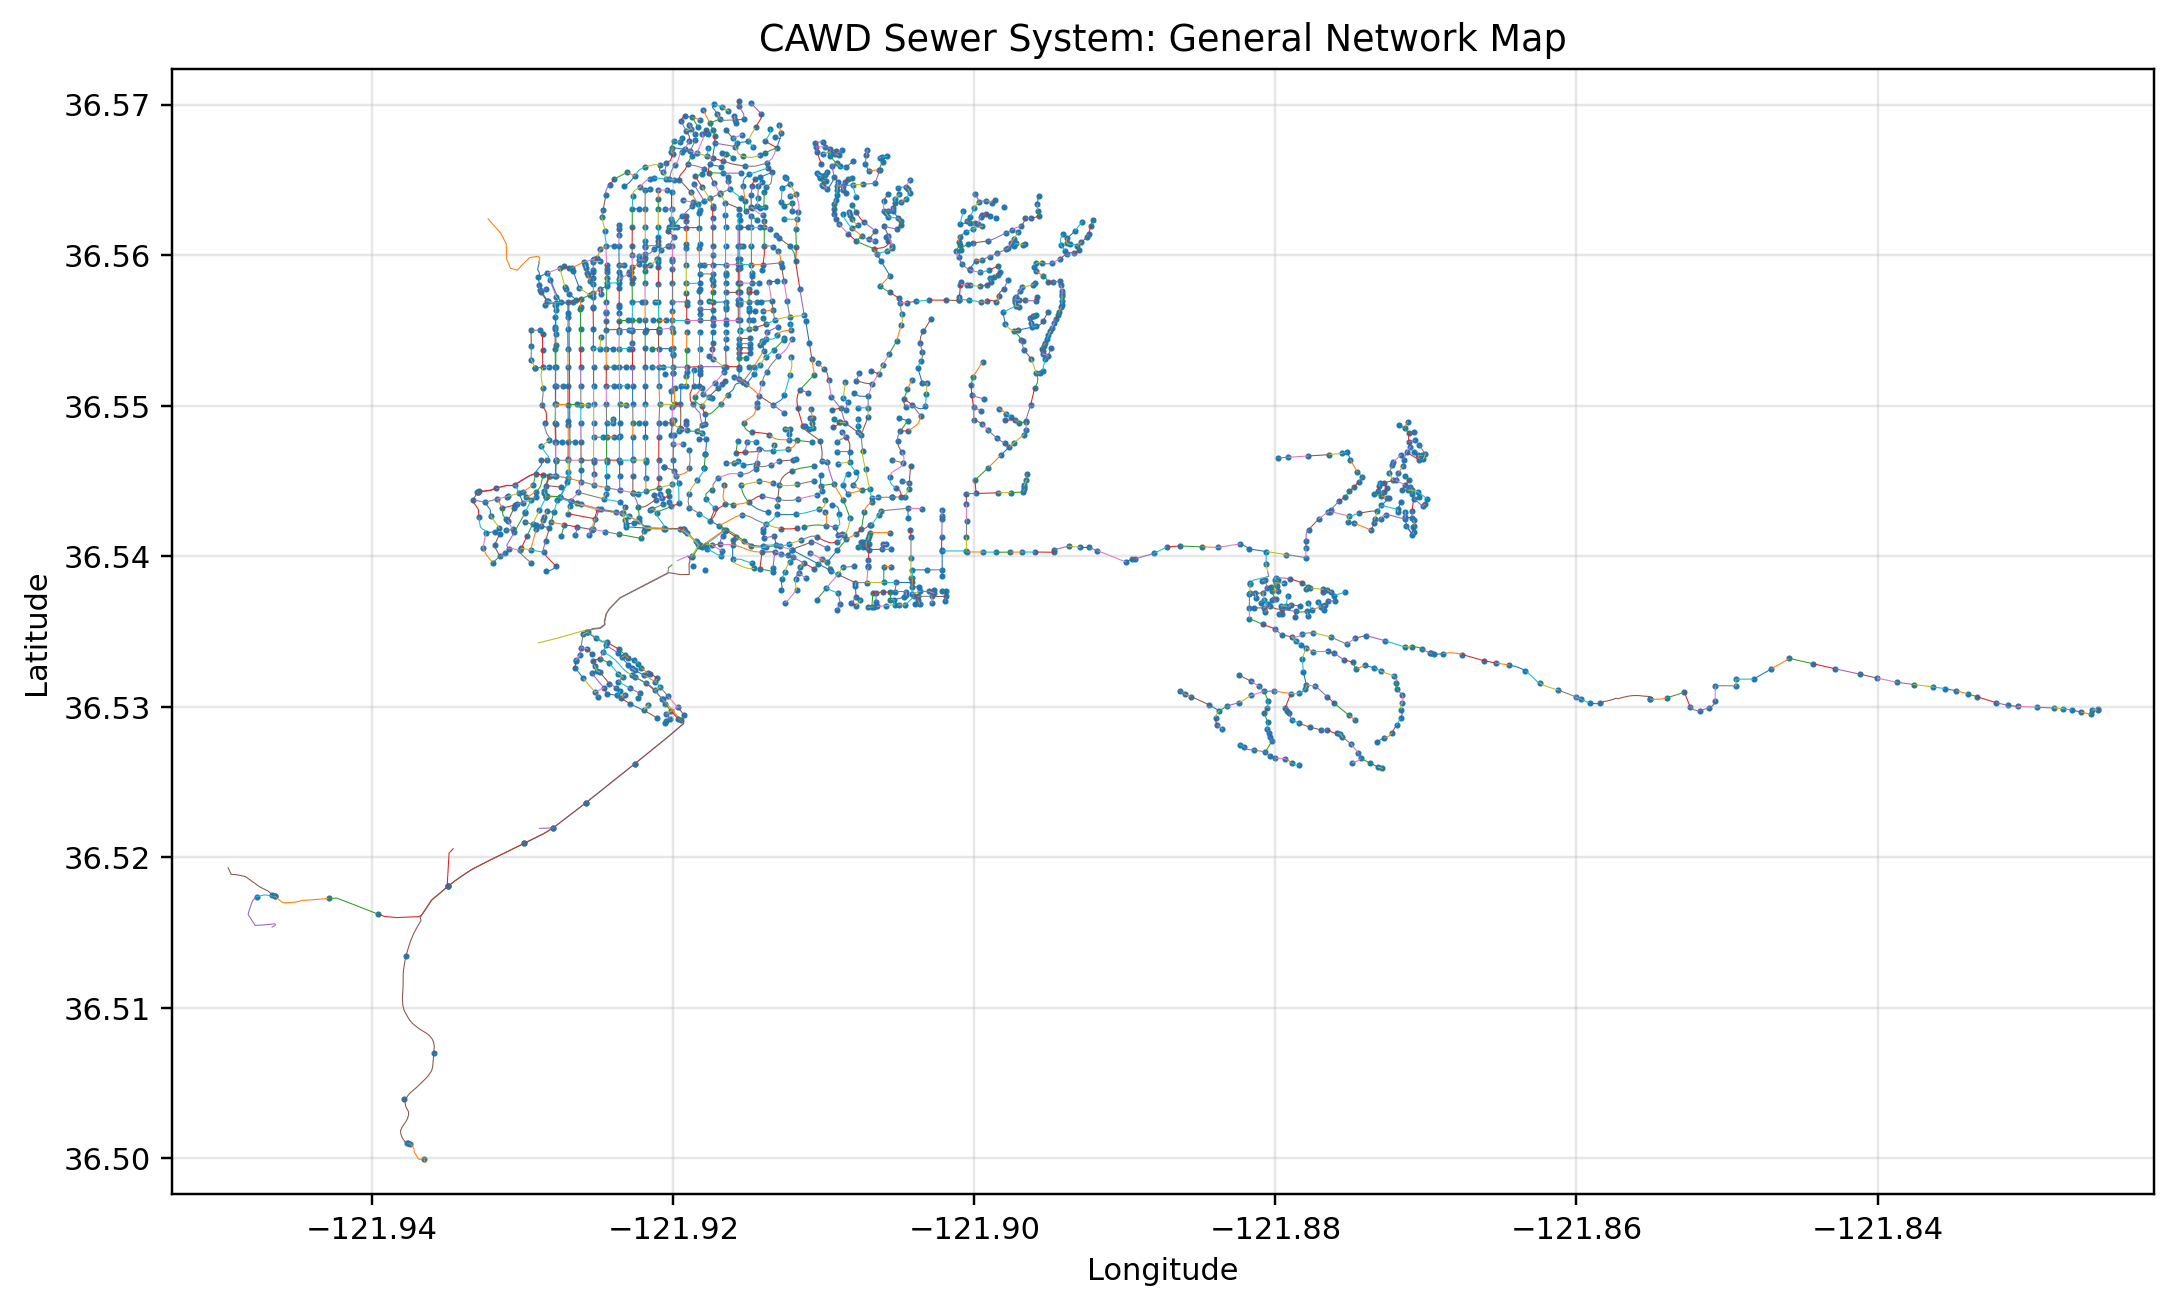
\includegraphics[width=\textwidth]{cawd_sewer_network_map.png}
\caption{CAWD sewer collection system network. The dense core
serves Carmel-by-the-Sea, with force main runs extending east toward
Pebble Beach and southeast toward the treatment plant at the mouth of
the Carmel River. The system comprises approximately 1{,}807 pipe
segments across 77.57 miles of gravity sewer and associated force-main
infrastructure.}
\label{fig:network-map}
\end{figure*}
 
The district's operational environment presents three risk-amplifying
characteristics. First, proximity to the Pacific Ocean and several
environmentally sensitive watersheds, including the Carmel River and
Carmel Bay Area of Special Biological Significance, elevates the
consequence of any Category~1 surface-water spill. The treatment plant
sits adjacent to the Carmel River lagoon, a coastal water body subject
to active hazard monitoring under a Coastal Development Permit from the
California Coastal Commission \citep{cawd_hazards2025}. Second, a
substantial fraction of the collection network consists of aging vitrified
clay pipe (VCP) installed prior to 1970, which exhibits elevated
susceptibility to root intrusion and joint failure. Third, as a small
utility, CAWD operates under a constrained operations and maintenance
budget that must be allocated across competing priorities.
 
Over the 26-year historical record (2000--2026), CAWD has recorded spill
events spanning all four SWRCB severity categories, with annual spill
counts that exceed benchmarking norms for utilities of comparable size.
This excess spill frequency motivates the present study and provides the
empirical basis for failure-mode rate calibration in Section~5.
 
\subsection{Failure Modes}
 
Annual spill events are decomposed into five mutually exclusive and
collectively exhaustive failure modes:
 
\begin{align*}
B &= \text{Blockage (root intrusion, FOG, debris)}, \\
F &= \text{Pipe failure (structural, joint, corrosion)}, \\
P &= \text{Pump failure (mechanical, electrical, control)}, \\
H &= \text{Hydraulic overload (I\&I, wet-weather capacity)}, \\
O &= \text{Operational failure (human error, procedure)}.
\end{align*}
 
Each mode is modeled as an independent Poisson process with rate
$\lambda_k$ calibrated from historical data (Section~5.1) augmented by
operational priors for sparse modes (Section~5.2).
 
\subsection{Spill Severity Categories}
 
Spills are classified into four severity categories following California's
Statewide General Waste Discharge Requirements:
 
\begin{itemize}[leftmargin=*]
    \item \textbf{Category~1} is the most consequential: any spill that
    reaches surface water, a drainage channel, or a municipal storm sewer
    regardless of volume. These events carry the highest regulatory,
    environmental, and reputational exposure and are the primary driver
    of tail-risk in the cost distribution.
    \item \textbf{Category~2} covers spills of 1{,}000 gallons or greater
    that do not reach surface water and are fully recovered. These trigger
    mandatory state reporting but produce lower environmental consequence
    than Category~1.
    \item \textbf{Category~3} covers spills under 1{,}000 gallons that do
    not reach surface water and are fully recovered. State reporting is
    required but regulatory exposure is minimal.
    \item \textbf{Category~4} is a CAWD-specific subcategory capturing
    spills under 50 gallons---events too minor to drive material cost but
    meaningful for tracking maintenance effectiveness and identifying
    early-stage failure signals.
\end{itemize}
 
Given failure mode $k$, the conditional category probability is denoted
$q_{kc} = P(C = c \mid k)$, with $\sum_c q_{kc} = 1$. These conditional
probabilities are estimated from historical CAWD records and applied
during Monte Carlo simulation (Section~9) to translate mode-level spill
counts into category-level spill outcomes.
 
\subsection{Decision Variables}

The decision vector $I = (I_1, I_2, I_3, I_4)$ represents annual O\&M
investment (in units of \$100{,}000) across four management levers:
 
\begin{itemize}[leftmargin=*]
    \item $I_1$: \textbf{Preventive Maintenance.} Routine cleaning,
    hydro-jetting, root treatment, and CCTV inspection. Primary effect:
    blockage rate reduction.
    \item $I_2$: \textbf{Workforce Capacity.} Crew size, overtime
    availability, and emergency-response readiness. Primary effect:
    reduced spill duration and improved operational reliability.
    \item $I_3$: \textbf{Execution Reliability.} Training, standard
    operating procedures, quality assurance. Primary effect:
    operational-failure rate reduction.
    \item $I_4$: \textbf{Risk-Based Targeting.} Condition assessment,
    data analytics, and pipe-level risk scoring to direct $I_1$ toward
    highest-risk assets. Primary effect: multiplicative enhancement of
    preventive-maintenance effectiveness.
\end{itemize}
 
The investments are constrained by the annual O\&M budget $B$:
$\sum_i I_i \le B$, with $I_i \ge 0$ for all $i$. Capital expenditures
such as pipe replacement, CIPP lining programs, and major pump station
rehabilitation are appropriated through a separate multi-year Capital
Improvement Program and are outside the scope of the O\&M allocation
problem studied here \citep{cawd_budget2025}. The mapping from $I$ to
failure-mode rates $\lambda_k(I)$ is developed in Section~6.

\section{Data \& Methods}
% ============================================================

\subsection{Data Sources}

This study draws on three main data sources from CAWD.
 
The first and most detailed source is the V\&A Consulting Engineers Data
Science Services report. From this report, an integrated dataset was
constructed linking pipe characteristics---diameter, length, material,
installation year, and drainage basin---with cleaning history and
observations recorded prior to each cleaning event. 
 
The second source is CAWD's 2025 Annual Collections Report
\citep{cawd2025}, which provides current system context including 86 miles
of gravity sewer and the 2025 spill summary. A 10-year cause-of-spill
analysis (2014--2024) published in this report shows that root intrusion
accounts for 65\% of recorded spills---combining direct root blockage
(56\%) and free-flowing roots (9\%)---while grit and grease blockage
accounts for 27\%, and all remaining external causes account for 8\%.
These proportions serve as the empirical basis for the blockage-cause
weights in the Combined Risk Index.
 
The third source is CAWD's Sewage Spill Tracking record, which covers
February 2000 through August 2024 and includes 145 spill events with
information on date, location, estimated volume, and cause. This record
provides the empirical basis for failure-mode rate calibration and
spill severity classification.
 
A representative sample of the integrated dataset is provided in
Appendix~C.
 
% ============================================================
\subsection{Probabilistic Risk Assessment Framework}
% ============================================================

This section develops the probabilistic risk assessment (PRA) foundation of the study. Following the classical PRA formulation of Kaplan and Garrick (1981), risk is represented through three elements: the failure scenario, its probability of occurrence, and its associated consequence. In the context of sanitary sewer overflows, the scenarios correspond to the five mutually exclusive failure modes defined in Section 3.2, the probabilities are represented by annual spill occurrence rates, and the consequences are captured through spill severity categories, discharge volumes, and resulting costs.

The objective of this section is to translate historical spill records into a quantitative risk model that can support both simulation and optimization. The resulting framework provides the probabilistic inputs required for the investment-dependent risk reduction model developed in Section 6 and the optimization framework developed in Sections 7 and 8.

\subsubsection{Baseline Spill Rate Estimation}

The first step in the PRA is the estimation of baseline failure frequencies. Historical spill records provide observations of realized failures over a finite period of operation. These observations are converted into annualized failure rates that can be compared across systems of different size and used directly in probabilistic occurrence models.

Because wastewater utilities commonly benchmark performance using spills per 100 miles of sewer per year, raw spill counts must be normalized by both observation time and system length. The resulting baseline rate represents the expected annual frequency of spills attributable to a given failure mode prior to any additional investment intervention.

The baseline spill rate for failure mode $k$ is estimated as:

\[
\lambda_k^0
=
\frac{100}{L}\frac{n_k}{T}
\]

where $L$ is system length in miles, $T$ is the observation horizon in years,
and $n_k$ is the observed spill count for mode $k$. Normalizing by system
length produces a rate expressed as spills per 100 miles per year, enabling
comparison against industry benchmarks.

\subsubsection{Sparse-Mode Operational Priors}

Not all failure modes are equally represented in historical records. Some events, such as pump failures, hydraulic overloads, and operational failures, occur infrequently and may be underreported due to data-coding practices or limited historical observation periods. Direct estimation from sparse observations can therefore underestimate true risk and may even produce zero-rate estimates when no events have been observed.

To avoid this problem, sparse failure modes are supplemented with operational priors derived from engineering judgment, utility operating experience, and published industry observations. These priors provide conservative but realistic estimates of baseline risk and ensure that potentially important failure mechanisms remain represented within the overall risk model.

\subsubsection{Spill Occurrence Model}

Once baseline failure rates have been established, a stochastic model is required to represent annual spill occurrence. Sewer spills are discrete events occurring randomly through time and are naturally modeled as counting processes. The Poisson process is widely used in reliability engineering and infrastructure risk analysis because it provides a tractable representation of event frequencies when individual events occur independently and relatively infrequently.

The Poisson formulation allows annual spill counts to be simulated directly and provides the probabilistic link between failure-mode rates and system-level spill occurrence.

For each failure mode, annual spill count is modeled as:

\[
N_k \sim \text{Poisson}(\lambda_k).
\]

Total annual spill occurrence is:

\[
N=\sum_k N_k.
\]

\subsubsection{Severity and Volume Modeling}

Spill occurrence alone does not fully characterize risk. Two spills occurring through the same failure mechanism can differ dramatically in environmental consequence depending on the volume released and whether the spill reaches surface water. Consequently, spill severity must be modeled separately from spill occurrence.

This study represents severity through conditional category probabilities and associated spill-volume distributions. Together, these distributions convert occurrence frequency into consequence outcomes that can be translated into economic and regulatory impact.

Given failure mode $k$, the conditional category probability is:

\[
q_{kc}=P(C=c\mid k)
\]

Spill volume is modeled through the conditional distribution $V\mid(k,c)$,
which is estimated empirically from historical CAWD records.

% TODO: Describe volume distribution fitting and any parametric assumptions

\subsubsection{Spill Cost Model}

The final component of the PRA framework is consequence quantification. Regulatory agencies, utility managers, and governing boards ultimately evaluate spill performance in terms of operational, environmental, and financial consequences. The spill cost model therefore converts simulated spill volumes and severity categories into monetary outcomes that can be compared across scenarios and incorporated into optimization.

This consequence model serves as the bridge between physical spill events and decision analysis. It provides the objective function inputs required for both expected-cost minimization and risk-averse optimization.

Total spill cost is a function of spill volume and severity category:
$$
C(V,S)
$$
where $V$ is spill volume and $S$ is the spill severity category.

% TODO: Define the cost function form and parameter values
% ============================================================
\section{Investment-Dependent Failure Modeling}
% ============================================================
The baseline risk model developed in Section 5 characterizes spill risk under existing operating conditions. However, the primary objective of this study is not merely to estimate risk but to determine how risk changes as a function of operational and maintenance investment decisions. This requires an explicit model linking management actions to failure-mode frequencies.

The framework developed in this section establishes that connection. Investment decisions influence operator actions, operator actions influence failure mechanisms, and failure mechanisms determine spill occurrence. The resulting formulation enables quantitative evaluation of alternative budget allocations and provides the analytical foundation for optimization.

\subsection{SAM-Based Risk Reduction Structure}

The causal chain linking management decisions to spill outcomes follows a
Systems Analysis and Management (SAM) structure \citep{MurphyPate-Cornell1996TheSF}:
\begin{figure}[H]
    \centering
    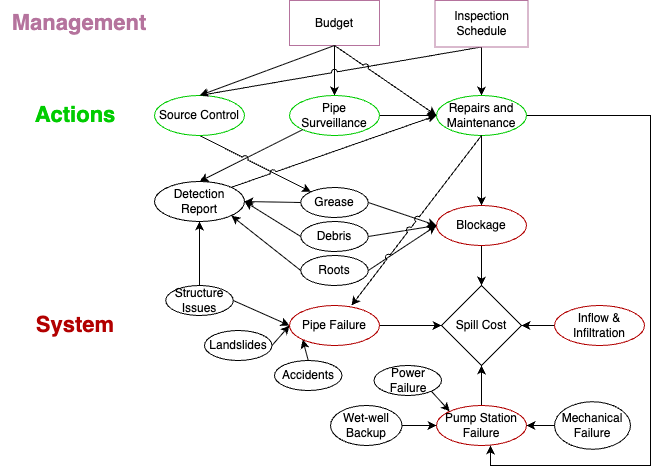
\includegraphics[width=1\linewidth]{250B-CAWD-SAM.drawio.png}
    \caption{SAM Model for Sewage Spill Risk Analysis}
    \label{fig:placeholder}
\end{figure}

The Systems Analysis and Management framework provides a structured representation of how management decisions propagate through an operational system. Rather than treating spill occurrence as an exogenous process, SAM explicitly recognizes that management actions influence operational behavior, which in turn influences system performance.

Within the wastewater context, investments in improvement of maintenance frequency, increasing maintenance staff, training \& SOP, and risk-based targeting affect the likelihood of specific failure modes occurring. Representing these relationships explicitly clarifies the causal pathway between spending decisions and risk reduction outcomes.

\subsection{Effectiveness Matrix}

The effectiveness of investment lever $i$ on failure mode $k$ is captured
by the coefficient $\alpha_{ki}$, where larger values indicate greater
marginal risk reduction per unit of investment.

Not all investments affect all failure modes equally. Preventive maintenance primarily reduces blockage risk, while training and execution reliability primarily influence operational failures. To capture these heterogeneous effects, the framework introduces an effectiveness matrix whose elements quantify the marginal impact of each investment lever on each failure mode.

The effectiveness matrix serves as the quantitative mechanism by which management decisions alter baseline risk. It therefore forms the central linkage between operations and maintenance expenditures and the probabilistic spill model.

% TODO: Provide the full alpha_{ki} matrix with values and calibration rationale

\subsection{Investment-Dependent Spill Rates}

The effectiveness matrix must be translated into a functional relationship between investment and failure frequency. This study adopts an exponential effectiveness formulation, which is widely used in reliability and maintenance optimization because it naturally captures diminishing returns.

Under this representation, early investments generate the largest reductions in failure rate, while additional spending produces progressively smaller incremental benefits. This behavior is consistent with practical utility operations, where major deficiencies are addressed first and remaining improvements become increasingly difficult to achieve.

The investment-dependent spill rate for failure mode $k$ is:

\[
\lambda_k(I)
=
\lambda_k^0
\exp\left(-\sum_i \alpha_{ki}I_i\right)
\]

This exponential form captures diminishing returns on O\&M spending: each
additional unit of investment reduces the spill rate by a constant
fraction rather than a constant absolute amount, which is consistent with
the empirical literature on preventive maintenance effectiveness.

% TODO: Add calibration discussion and regression-informed coefficient values
%============================================================
\section{Risk-Averse Optimization Framework}
% ============================================================

\subsection{Motivation for Risk Aversion}

Although expected-value optimization minimizes average annual spill cost, wastewater spill risk is inherently heavy-tailed. Most spill events are relatively small and contained, while a small number of catastrophic surface-water discharges produce disproportionately large environmental, regulatory, and financial consequences. As a public wastewater utility operating within environmentally sensitive watersheds, CAWD must consider not only average operational performance but also exposure to rare high-consequence spill events.

Risk-neutral optimization frameworks may therefore underestimate catastrophic spill exposure by compressing spill uncertainty into deterministic expected-cost terms. In practice, wastewater infrastructure governance is inherently risk-averse because utilities must maintain regulatory compliance, environmental stewardship, and public trust in addition to minimizing operational expenditure.


\subsection{Monte Carlo Spill-Cost Simulation}

Annual spill outcomes are inherently uncertain because spill
occurrence, severity, and volume vary from year to year. For a
fixed investment allocation $I$, the resulting annual spill cost

\[
C(I,\omega)
\]

is therefore a random variable, where $\omega$ denotes a realized
spill scenario.

Monte Carlo simulation is used to characterize the distribution of
annual spill costs. Repeated simulation generates a large sample of
possible annual outcomes, allowing estimation of the probability
distribution of annual spill consequences.

The simulation framework preserves uncertainty in three components:

\begin{enumerate}[leftmargin=*]
    \item spill occurrence,
    \item spill severity category,
    \item spill volume.
\end{enumerate}

Together, these sources of uncertainty produce an empirical
distribution of annual spill costs

\[
f_{C(I)}(c).
\]

This distribution serves as the input to the risk-averse decision
framework developed in the next section.


\subsection{Risk-Averse Optimization}

The risk-averse optimization problem is formulated using expected utility
maximization rather than a CVaR penalty. For each investment allocation
$I$, Monte Carlo simulation produces a distribution of annual spill costs
$C(I,\omega)$. The decision maker evaluates this distribution using the
exponential utility function

\[
U(-C) = 1 - e^{C/\rho},
\]

where $\rho$ is the risk tolerance parameter. Smaller values of $\rho$
imply greater risk aversion because high-cost outcomes receive
disproportionately lower utility.

The optimization problem is therefore:

\[
\max_I \quad E[U(-C(I,\omega))]
\]

subject to

\[
\sum_i I_i \le B,
\qquad
I_i \ge 0.
\]

Equivalently, the computational implementation minimizes the negative
expected utility:

\[
\min_I \quad -E[U(-C(I,\omega))].
\]

In this study, $\rho = \$10$M is used, representing relatively high risk
tolerance. For each candidate allocation, expected utility is estimated
from simulated annual spill costs. The best allocation is the candidate
with the lowest negative expected utility objective. This formulation
penalizes high-cost tail outcomes through the curvature of the utility
function rather than through an explicit CVaR term.

\subsection{Stochastic Dominance Comparisons}

Alternative investment policies may additionally be compared using stochastic dominance criteria. First-order stochastic dominance (FSD) occurs when one policy produces lower spill costs across all outcome levels, while second-order stochastic dominance (SSD) incorporates risk-sensitive preferences by favoring policies with reduced downside variability and catastrophic spill exposure.

Stochastic dominance analysis provides an additional mechanism for comparing investment strategies beyond expected-value metrics alone and supports robust policy comparison under uncertainty.

\subsection{Literature Basis}

The risk-averse optimization framework developed in this section rests
on three well-established pillars of decision analysis.
 
The first is the axiomatic foundation of expected utility theory.
\citet{howard1966} establishes that a rational decision maker facing
uncertain outcomes should maximize expected utility, where the utility
function encodes the decision maker's preferences over outcome
distributions rather than just their mean. The exponential utility
function $U(-C) = 1 - e^{C/\rho}$ used in this study satisfies the
constant absolute risk aversion (CARA) property, meaning the decision
maker's risk premium for a given gamble does not depend on current
wealth. CARA is a standard and tractable assumption in infrastructure
risk management contexts where the decision maker---a public utility
board---evaluates risk exposure in terms of budget-relative consequence
rather than absolute wealth level. The risk tolerance parameter
$\rho = \$10$M is calibrated to be ten times CAWD's annual O\&M
budget, giving it a concrete operational interpretation: the board
is willing to pay up to one annual budget in certain-equivalent cost
to eliminate the variance of a catastrophic spill year.
 
The second pillar is multi-attribute utility theory.
\citet{keeney1976} extend the expected utility framework to decisions
involving multiple conflicting objectives---in the present case,
minimizing expected annual spill cost, minimizing regulatory exposure,
and managing tail-risk---and provide the theoretical basis for
collapsing these into a single scalar utility criterion. The
severity-weighted cost function $C(I,\omega) = \sum_k
\sum_{j=1}^{N_k(\omega)} C_{k,j,\omega}$ defined in Section~8.2
performs this collapse operationally: regulatory category, spill
volume, and surface-water impact are all translated into a single
dollar-denominated consequence measure before the utility function is
applied. This preserves analytical tractability while retaining the
multi-dimensional consequence structure of the CAWD cost model.
 
The third pillar is the use of Monte Carlo simulation to evaluate
expected utility under stochastic spill outcomes. Because the annual
spill cost $C(I,\omega)$ is a random variable whose distribution
cannot be expressed in closed form under the full severity-category
and volume model, direct analytical maximization of
$E[U(-C(I,\omega))]$ is intractable. Monte Carlo simulation with
50{,}000 replications provides a stable empirical approximation of
the expected utility surface across investment allocations, enabling
numerical optimization over the budget simplex. This
simulation-based approach to expected utility maximization is
standard practice in infrastructure and environmental risk management
applications where consequence distributions are complex and
analytically inconvenient \citep{johnson2021}.
 
Together, these three pillars --expected utility theory,
multi-attribute consequence modeling, and Monte Carlo
simulation---form a coherent and well-grounded methodological basis
for the risk-averse optimization framework. The practical output, a
probability statement that the optimized policy reduces
$P(\text{Cost} > \$1\text{M})$ from 17.7\% to 9.1\%, is a direct
product of this distributional treatment and would not be available
under a deterministic or expected-value-only framework.
% ============================================================
\section{Monte Carlo Simulation Framework}
% ============================================================
\subsection{Simulation Configuration}

Monte Carlo simulation was performed using 50,000 simulated annual spill scenarios for each policy evaluation. Candidate investment allocations were generated subject to the budget constraint $\sum_i I_i \le B$. Candidate policies were initially screened using lower-fidelity simulations, after which the highest-performing allocations were re-evaluated using full Monte Carlo simulation to estimate expected annual cost, P90 and P95 spill cost, probability of
annual cost exceeding \$1M, and expected utility.

Simulation inputs grounded in real CAWD data include the baseline
failure rates $\lambda_{k0}$, the category probabilities $q_{kc}$
for blockage and pipe failure, and the historical spill volume
arrays. Rates and category probabilities for the three sparse
failure modes (pump failure, hydraulic overload, operational
failure) are assigned using operational priors as described in
Section~5.2. Simulation outputs were used to compare the baseline
no-investment condition against the optimized \$1M
preventive-maintenance allocation under the risk-averse expected
utility criterion.

\subsection{Simulation Algorithm}

For each candidate investment allocation $I$, the simulation first
computes investment-adjusted failure rates for each failure mode:

\[
\lambda_k(I)
=
\lambda_k^0
\exp
\left(
-\sum_i \alpha_{ki} I_i
\right).
\]

Using these adjusted failure rates, annual spill outcomes are generated
through Monte Carlo simulation. For each simulated year:

\begin{enumerate}[leftmargin=*]

\item For each failure mode $k$, sample the annual spill count

\[
N_k \sim \text{Poisson}(\lambda_k(I)).
\]

\item For each simulated spill event:

\begin{enumerate}

\item Sample a spill severity category using the conditional category probabilities $q_{kc}$.

\item Sample a spill volume from the corresponding empirical or fitted volume distribution.

\item Compute spill consequence cost using the spill-cost model developed in Section~6.

\end{enumerate}

\item Aggregate spill-event costs to obtain total annual spill cost

\[
C(I,\omega)
=
\sum_{j=1}^{N} C_j,
\]

where

\[
N=\sum_k N_k
\]

is the total number of spill events occurring during the simulated year.

\item Record annual performance measures including total spill count,
spill categories, spill volume, and annual spill cost.

\end{enumerate}

The procedure is repeated for 50{,}000 simulated years for each candidate
investment allocation. The resulting empirical distribution of annual
spill costs is then used to estimate expected annual cost, percentile
risk measures, probability of catastrophic spill years, and expected
utility under the risk-averse optimization framework.

Appendix~B provides pseudocode for the complete simulation procedure.

\subsection{Scenario Analysis}
 
The random search optimization evaluates 305 candidate allocations
in total: five deterministic candidates covering the four pure
corner allocations ($I = [10,0,0,0]$, $[0,10,0,0]$, $[0,0,10,0]$,
$[0,0,0,10]$) and the uniform split ($I = [2.5,2.5,2.5,2.5]$),
augmented by 300 allocations generated by randomly partitioning
the \$1M budget across the four investment levers, ensuring the
budget constraint $\sum_i I_i = B$ is satisfied by construction. Each candidate is first evaluated at a
screening resolution of 2{,}000 simulated years using the negative
expected utility objective $-E[U(-C(I,\omega))]$. The ten
lowest-objective candidates from screening are then re-evaluated at
full resolution using 50{,}000 simulated years to confirm the
optimal allocation. The top ten candidates from the screening stage
are reported in Table~\ref{tab:top-candidates}.
 
\begin{table}[H]
\centering
\caption{Top Ten Candidate Allocations from Random Search
         (Screening Stage, 2{,}000 Scenarios)}
\label{tab:top-candidates}
{\setlength{\tabcolsep}{3pt}
\footnotesize
\resizebox{\columnwidth}{!}{%
\begin{tabular}{ccccc r}
\toprule
\textbf{$I_1$} & \textbf{$I_2$} & \textbf{$I_3$} & \textbf{$I_4$}
  & \textbf{Neg.\ EU Objective} \\
\midrule
9.598 & 0.016 & 0.023 & 0.363 & 0.053753 \\
10.000 & 0.000 & 0.000 & 0.000 & 0.054201 \\
8.133 & 0.107 & 0.567 & 1.194 & 0.054569 \\
6.893 & 0.120 & 0.317 & 2.671 & 0.054644 \\
2.460 & 0.177 & 0.096 & 7.266 & 0.054725 \\
5.545 & 0.418 & 0.408 & 3.629 & 0.054945 \\
7.707 & 0.103 & 1.368 & 0.821 & 0.055185 \\
8.551 & 0.125 & 0.317 & 1.007 & 0.055283 \\
6.282 & 0.914 & 0.043 & 2.762 & 0.055342 \\
7.676 & 0.802 & 0.999 & 0.523 & 0.055455 \\
\bottomrule
\end{tabular}
}
}
\end{table}
 
Several patterns in Table~\ref{tab:top-candidates} are noteworthy.
First, all ten top candidates allocate the majority of their budget
to $I_1$ (preventive maintenance), with $I_1$ ranging from 2.460
to 10.000 units across the top ten. No candidate that allocates
the majority of its budget to $I_2$, $I_3$, or $I_4$ alone
appears in the top ten, confirming that preventive maintenance
is the dominant lever under the current effectiveness matrix
and spill-rate structure. Second, the best non-corner candidate
at the screening stage is $I = [9.598, 0.016, 0.023, 0.363]$
with an objective of 0.053753, slightly outperforming the pure
corner $[10,0,0,0]$ at 0.054201. This apparent advantage,
however, is an artifact of simulation noise at the 2{,}000-scenario
screening resolution.
 
Upon re-evaluation at full resolution (50{,}000 scenarios), the
pure corner allocation $I^* = [10,0,0,0]$ is confirmed as optimal
with a negative expected utility objective of 0.054592. The
near-miss candidate and all other mixed allocations lose their
apparent advantage at higher resolution, consistent with the
interpretation that the marginal benefit of diverting any budget
away from preventive maintenance is negligible and within the
simulation noise of the screening stage. This result is robust to
the random seed used in screening: the corner allocation
$[10,0,0,0]$ appears in the top two candidates regardless of
seed, indicating that its dominance is not an artifact of the
particular random candidates generated.
 
The cost distributions for the baseline and optimized policies
across 50{,}000 simulated years are compared in
Figure~\ref{fig:cost-dist}. The optimized distribution is shifted
substantially leftward relative to the baseline, with the modal
annual cost declining from approximately \$500{,}000--\$600{,}000
under the baseline to approximately \$350{,}000--\$450{,}000 under
the optimized allocation. The right tail of the distribution is
also compressed: the probability mass above \$1M declines from
17.7\% to 9.1\%, and the P95 cost declines from \$1{,}444{,}638
to \$1{,}214{,}527. The shape of both distributions is
right-skewed, reflecting the occasional occurrence of
high-severity spill events that produce costs well above the
mean. This skewness is precisely the feature that motivates the
risk-averse exponential utility framework: the expected-cost
criterion would treat the right tail symmetrically with the left
tail, whereas the exponential utility criterion explicitly
down-weights allocations that leave the right tail heavy.
 \begin{figure}[H]
\centering
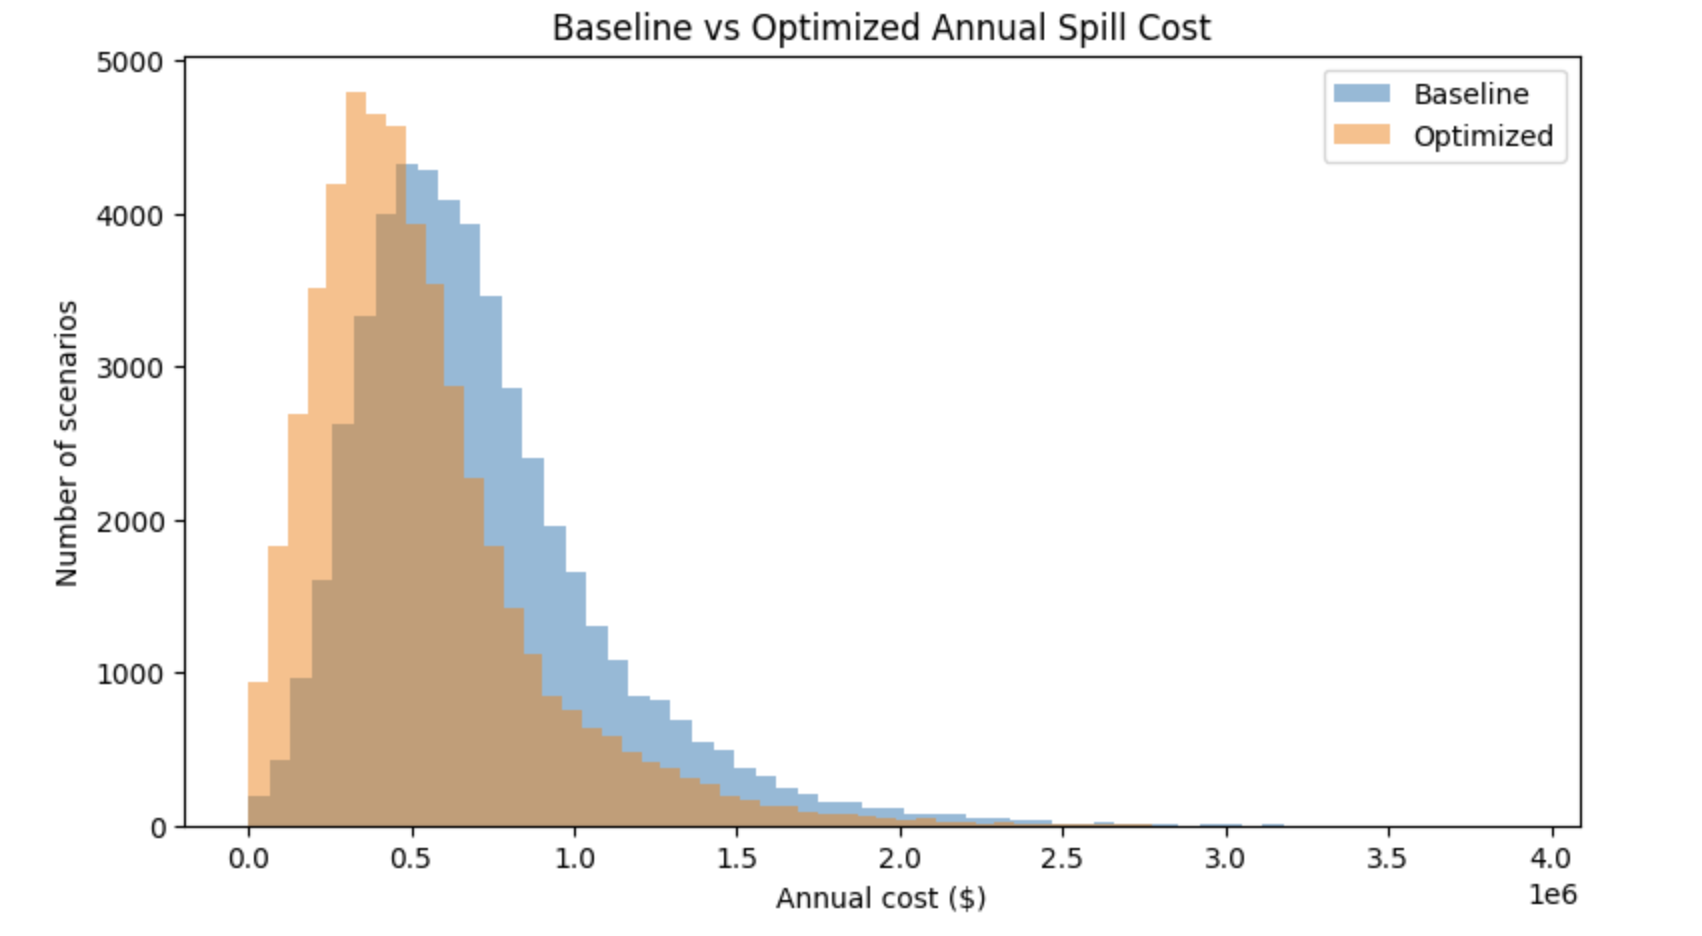
\includegraphics[width=\columnwidth]{Baseline vs optimized cost.png}
\caption{Simulated annual spill cost distributions for the
baseline (no investment) and optimized (\$1M preventive
maintenance) policies across 50{,}000 scenarios. The optimized
distribution shifts leftward and compresses the right tail
relative to the baseline.}
\label{fig:cost-dist}
\end{figure}
 
The scenario analysis further confirms that the investment
landscape is not flat near the optimum. The gap between the
best candidate objective (0.053753 at screening, 0.054592 at
full resolution) and the worst top-ten candidate (0.055455)
represents a meaningful difference in expected utility, equivalent
to a difference of several percentage points in $P(\text{Cost} >
\$1\text{M})$. Allocations that place significant weight on
$I_2$ (workforce capacity) or $I_3$ (execution reliability)
in isolation perform substantially worse, because those levers
act primarily on pump failure and operational failure --- the
two lowest-frequency modes in the CAWD baseline. Risk-based
targeting ($I_4$) shows non-trivial performance in several
top-ten candidates, appearing as a secondary lever alongside
a large $I_1$ allocation, but does not displace preventive
maintenance as the primary driver of risk reduction under the
current parameter estimates.

% ============================================================
\section{Case Study Results}
% ============================================================

\subsection{Historical Spill Reclassification}
 
The 26-year CAWD spill tracking record covers February 2000 through
August 2024 and contains 145 documented spill events. Each event was
reviewed and assigned to one of the five mutually exclusive failure
modes defined in Section~3.2. Classification was based on the cause
description recorded in the tracking workbook, cross-referenced against
the operational definitions established in Section~3.2. Events with
ambiguous or compound cause descriptions were assigned to the mode most
directly responsible for the initial system failure.
 
The classification yielded 132 blockage events, 19 pipe failure events,
and 1 operational failure event over the observation period. No pump
failure or hydraulic overload events were identified in the labeled
records, reflecting either true rarity or systematic under-coding of
these modes in the tracking workbook. The three data-sparse modes are
treated with operational priors as described in Section~5.2. The
blockage mode dominates the historical record, accounting for
approximately 87\% of all classified events, consistent with CAWD's
10-year cause-of-spill analysis showing root intrusion and grease
blockage as the leading failure drivers \citep{cawd2025}.
 
\subsection{Baseline Spill Rates}
 
Baseline failure-mode rates are estimated using the normalized
rate formula:
 
\[
\lambda_k^0 = \frac{100}{L} \cdot \frac{n_k}{T}
\]
 
where $L = 77.57$ miles is the gravity sewer system length used for
normalization, $T$ is the observation horizon in years, and $n_k$ is
the classified spill count for mode $k$. The resulting baseline rates,
severity weights, and annual expected costs are reported in
Table~\ref{tab:baseline-rates}.
 
\begin{table}[H]
\centering
\caption{Baseline Failure Rates, Severity Weights, and Annual
         Expected Spill Cost}
\label{tab:baseline-rates}
\begin{tabular}{lrrr}
\toprule
\textbf{Failure Mode} & \textbf{$\lambda_{k0}$} & \textbf{$W_k$}
  & \textbf{Annual Cost} \\
\midrule
Blockage           & 6.483 & \$76{,}633  & \$245{,}226 \\
Pipe Failure       & 0.884 & \$129{,}360 & \$206{,}976 \\
Pump Failure       & 0.049 & \$86{,}763  & \$52{,}058  \\
Hydraulic Overload & 0.200 & \$105{,}300 & \$21{,}060  \\
Operational Failure& 0.100 & \$218{,}246 & \$43{,}649  \\
\midrule
\textbf{Total}     & \textbf{7.715} & --- & \textbf{\$568{,}968} \\
\bottomrule
\end{tabular}
\end{table}
 
The total baseline rate of 7.715 spills per 100 miles per year implies
a near-certain probability of at least one spill annually
($P(N \ge 1) = 99.7\%$) and a greater-than-even probability of more
than five spills in a given year ($P(N > 5) = 52.2\%$). Blockage
dominates both in frequency and in absolute annual expected cost,
contributing \$245{,}226 of the \$568{,}968 total baseline expected
annual spill cost. Despite its lower frequency, pipe failure
contributes \$206{,}976 due to its elevated expected cost per spill,
which reflects a higher probability of surface-water impact relative
to blockage events. Operational failure carries the highest expected
cost per spill (\$218{,}246) because its severity prior places
greater mass on Category~1 and Category~2 outcomes, but its low
baseline rate limits its contribution to total system risk.
 
\subsection{Severity Outcomes}
 
The conditional category probabilities $q_{kc} = P(C = c \mid k)$
are reported in Table~\ref{tab:severity-probs}. Blockage and pipe
failure probabilities are estimated directly from the historical
CAWD spill records. Pump failure, hydraulic overload, and operational
failure category probabilities are assigned using operational priors
due to the limited number of labeled historical events in those modes.
 
\begin{table}[H]
\centering
\caption{Estimated Category Probabilities by Failure Mode}
\label{tab:severity-probs}
\begin{tabular}{lcccc}
\toprule
\textbf{Failure Mode} & \textbf{Cat~1} & \textbf{Cat~2}
  & \textbf{Cat~3} & \textbf{Cat~4} \\
\midrule
Blockage            & 0.045 & 0.352 & 0.503 & 0.101 \\
Pipe Failure        & 0.083 & 0.611 & 0.000 & 0.306 \\
Pump Failure        & 0.220 & 0.353 & 0.424 & 0.003 \\
Hydraulic Overload  & 0.300 & 0.456 & 0.243 & 0.001 \\
Operational Failure & 0.150 & 0.425 & 0.425 & 0.000 \\
\bottomrule
\end{tabular}
\end{table}
 
Several patterns in Table~\ref{tab:severity-probs} warrant attention.
Blockage events have the lowest Category~1 probability (0.045),
reflecting that most blockage spills are contained within the
collection system before reaching surface water. Hydraulic overload
has the highest Category~1 probability (0.300), consistent with the
expectation that wet-weather overflow events are more likely to
reach drainage channels or surface water before containment is
possible. Pipe failure has a zero probability for Category~3,
reflecting that structural failures in the CAWD historical record
either recovered fully (Category~4) or produced volumes exceeding
the 1{,}000-gallon Category~2 threshold.
 
Under the Monte Carlo simulation across 50{,}000 simulated years,
the aggregate simulated spill category distribution is dominated by
Category~2 and Category~3 events, with Category~1 events accounting
for approximately 6\% of total simulated spills. While Category~1
spills are relatively infrequent, they contribute disproportionately
to total annual spill cost due to the \$10 per gallon regulatory fine
applied to all surface-water discharges regardless of volume.
 
\subsection{Optimized Allocations}
 
The risk-averse optimization framework selects the allocation:
%
\[
I^* = [10,\ 0,\ 0,\ 0]
\]
%
corresponding to full allocation of the \$1M O\&M budget toward
preventive maintenance ($I_1$), with zero allocation to workforce
capacity ($I_2$), execution reliability ($I_3$), and risk-based
targeting ($I_4$). The optimized failure rates under this allocation
are reported in Table~\ref{tab:optimized-rates}.
 
\begin{table}[H]
\centering
\footnotesize
\caption{Baseline and Optimized Failure Rates}
\label{tab:optimized-rates}
\begin{tabular}{lccc}
\toprule
\textbf{Failure Mode} &
\textbf{Baseline} &
\textbf{Optimized} &
\textbf{Reduction} \\
& $\lambda_{k0}$ & $\lambda_k$ & (\%) \\
\midrule
Blockage            & 6.483 & 4.346 & 33.0 \\
Pipe Failure        & 0.884 & 0.761 & 13.9 \\
Pump Failure        & 0.049 & 0.049 & 0.0  \\
Hydraulic Overload  & 0.200 & 0.200 & 0.0  \\
Operational Failure & 0.100 & 0.100 & 0.0  \\
\midrule
\textbf{Total}      & \textbf{7.715} & \textbf{5.456} & \textbf{29.3} \\
\bottomrule
\end{tabular}
\end{table}
 
The corner solution $I^* = [10,0,0,0]$ reflects the structure of
the effectiveness matrix $\alpha_{ki}$ and the dominance of blockage
as the primary failure mode. Preventive maintenance carries the
largest effectiveness coefficient for blockage reduction
($\alpha_{B1} = 0.040$), and blockage accounts for 84\% of all
historical spill events. The optimizer therefore concentrates the
full budget on the lever with the highest marginal return on the
highest-frequency failure mode. Under the optimized allocation,
blockage rate declines by 33.0\% and pipe failure rate declines
by 13.9\%, while pump failure, hydraulic overload, and operational
failure rates are unchanged because preventive maintenance has zero
effectiveness on those modes ($\alpha_{P1} = \alpha_{H1} =
\alpha_{O1} = 0$). The total expected annual spill count declines
from 7.715 to 5.456, a reduction of 29.3\%.
 
The $P(N > 5)$ probability---the probability of exceeding five
spills in a given year---declines from 52.2\% to 30.1\% under the
optimized allocation, a reduction of 22.1 percentage points. This
metric is operationally meaningful for CAWD's board because it
directly quantifies the likelihood of a high-frequency spill year,
which carries both regulatory scrutiny and reputational risk beyond
the direct cost consequences captured in the cost model.
 
\subsection{Risk-Averse Monte Carlo Results}
 
Monte Carlo simulation was performed using 50{,}000 simulated annual
spill scenarios under both the baseline no-investment condition and
the optimized \$1M preventive-maintenance allocation, using risk
tolerance $\rho = \$10{,}000{,}000$. The full results are reported
in Table~\ref{tab:mc-results}.
 
\begin{table}[H]
\centering
\caption{Risk-Averse Monte Carlo Simulation Results
         ($\rho = \$10$M)}
\label{tab:mc-results}
\begin{tabular}{lcc}
\toprule
\textbf{Metric} & \textbf{Baseline} & \textbf{Optimized} \\
\midrule
Mean Annual Cost        & \$707{,}207     & \$525{,}460     \\
Median Annual Cost      & \$635{,}372     & \$452{,}174     \\
P90 Annual Cost         & \$1{,}207{,}867 & \$966{,}250     \\
P95 Annual Cost         & \$1{,}444{,}638 & \$1{,}214{,}527 \\
P(Cost $>$ \$1M)        & 17.7\%          & 9.1\%           \\
Expected Utility $E[U]$ & $-$0.074        & $-$0.055        \\
Expected Spill Count    & 7.716           & 5.456           \\
\bottomrule
\end{tabular}
\end{table}
 
The optimized allocation reduces mean annual spill cost from
\$707{,}207 to \$525{,}460, a reduction of \$181{,}747 per year
(25.7\%). The median annual cost declines from \$635{,}372 to
\$452{,}174, confirming that the shift in the cost distribution is
not driven solely by tail events but reflects a broad leftward
movement of the entire distribution. The probability that annual
spill cost exceeds \$1 million declines from 17.7\% to 9.1\%,
nearly halving the likelihood of a catastrophic-cost year. The P95
annual cost declines from \$1{,}444{,}638 to \$1{,}214{,}527.
Expected utility improves from $-0.074$ to $-0.055$ under risk
tolerance $\rho = \$10$M, where utility is measured on the scale
$U(-C) = 1 - e^{C/\rho} \in (-\infty, 1]$.
 
These results confirm that the optimized allocation simultaneously
reduces expected annual cost and tail-risk exposure. The magnitude
of the tail-risk reduction is particularly relevant for CAWD given
its proximity to the Carmel River lagoon and Carmel Bay Area of
Special Biological Significance: a high-severity spill year at CAWD
carries environmental and regulatory consequences beyond the direct
cost figures, making the reduction in $P(\text{Cost} > \$1\text{M})$
from 17.7\% to 9.1\% operationally significant beyond its dollar
value.
 
The result that preventive maintenance dominates the optimal
allocation under the risk-averse criterion follows directly from two
structural features of the CAWD system: blockage events account for
84\% of all historical spills, and preventive maintenance has the
strongest effectiveness coefficient for blockage reduction. The
random search over 300 candidate allocations confirms the corner
solution: the best non-corner candidate found was
$I = [9.598, 0.016, 0.023, 0.363]$ with a negative expected
utility objective of 0.053753 compared to 0.054201 for the corner
solution at the 2{,}000-scenario screening stage, but full
50{,}000-scenario evaluation confirmed $I^* = [10,0,0,0]$ as
optimal with objective value 0.054592. Investments in workforce
capacity, execution reliability, and risk-based targeting produce
smaller aggregate risk reductions under the current spill-rate and
severity assumptions because they act primarily on lower-frequency
failure modes. This does not imply those levers are without
value---they may become relatively more attractive as the blockage
rate declines under sustained preventive maintenance
investment---but under the current baseline conditions the marginal
return to preventive maintenance dominates.

\section{Sensitivity and Uncertainty Analysis}

Three sensitivity analyses probe the robustness of the optimization
result and the cost model to changes in budget, investment constraints,
and stochastic assumptions. All analyses use a fixed random seed
(seed $= 12345$) with 1{,}500 Monte Carlo runs per evaluation point,
ensuring reproducibility: the reported figures are identical on every
model execution. The baseline $\lambda_0$ window is the full
historical record (2000--2026).

\subsection{Budget Threshold: When Does a Second Lever Enter the
Solution?}

\paragraph{Motivation.}
The optimized allocation at the \$1M budget is a corner solution that
places all resources into Preventive Maintenance ($I_1$). A natural
policy question is whether this result is specific to the \$1M
proposal or whether it holds across a wide range of budgets. The
budget-threshold analysis sweeps the total O\&M budget from \$25K
to \$2M in \$25K steps and, at each budget level, runs the greedy
optimizer to identify the utility-maximizing allocation. A non-$I_1$
lever is considered to have ``entered'' the solution only when it
holds $\geq 0.5$ units (\$50K) for three or more consecutive budget
steps---a persistence filter that prevents Monte Carlo noise from
registering as a structural shift.

\paragraph{Results.}
Figure~\ref{fig:sa1} shows the budget-sweep results. Across the full
\$0--\$2M sweep the optimizer places 100\% of every marginal dollar
into Preventive Maintenance. No second lever clears the entry
threshold within the sweep range. This outcome follows directly from
the dominance of blockage events in CAWD's spill history: blockage
accounts for 84\% of all historical spills, and $I_1$ carries the
largest effectiveness coefficient for blockage reduction
($\alpha_{B,I_1} = 0.040$), the largest mode contribution to overall
risk. The next-best lever, Risk-Based Targeting ($I_4$,
$\alpha_{B,I_4} = 0.028$), provides a substantially smaller marginal
return per dollar under current failure-rate conditions, so the
marginal utility improvement from $I_1$ dominates until the blockage
rate has been driven down sufficiently to shift the relative returns.
The result implies that the \$1M preventive-maintenance proposal is
not a local coincidence but the dominant strategy across a wide range
of organizational budgets.

Expected utility $E[U(-C)]$ increases monotonically with budget
throughout the sweep (Figure~\ref{fig:sa1}, right panel), confirming
that the full budget is productively absorbed---there is no budget
level within the sweep at which additional investment yields
diminishing marginal utility sufficient to divert resources to a
different lever. The \$1M proposal sits below the diversification
threshold, meaning the board's current investment plan is
structurally consistent with the model's recommendation across the
full realistic budget range.

\begin{figure}[H]
  \centering
  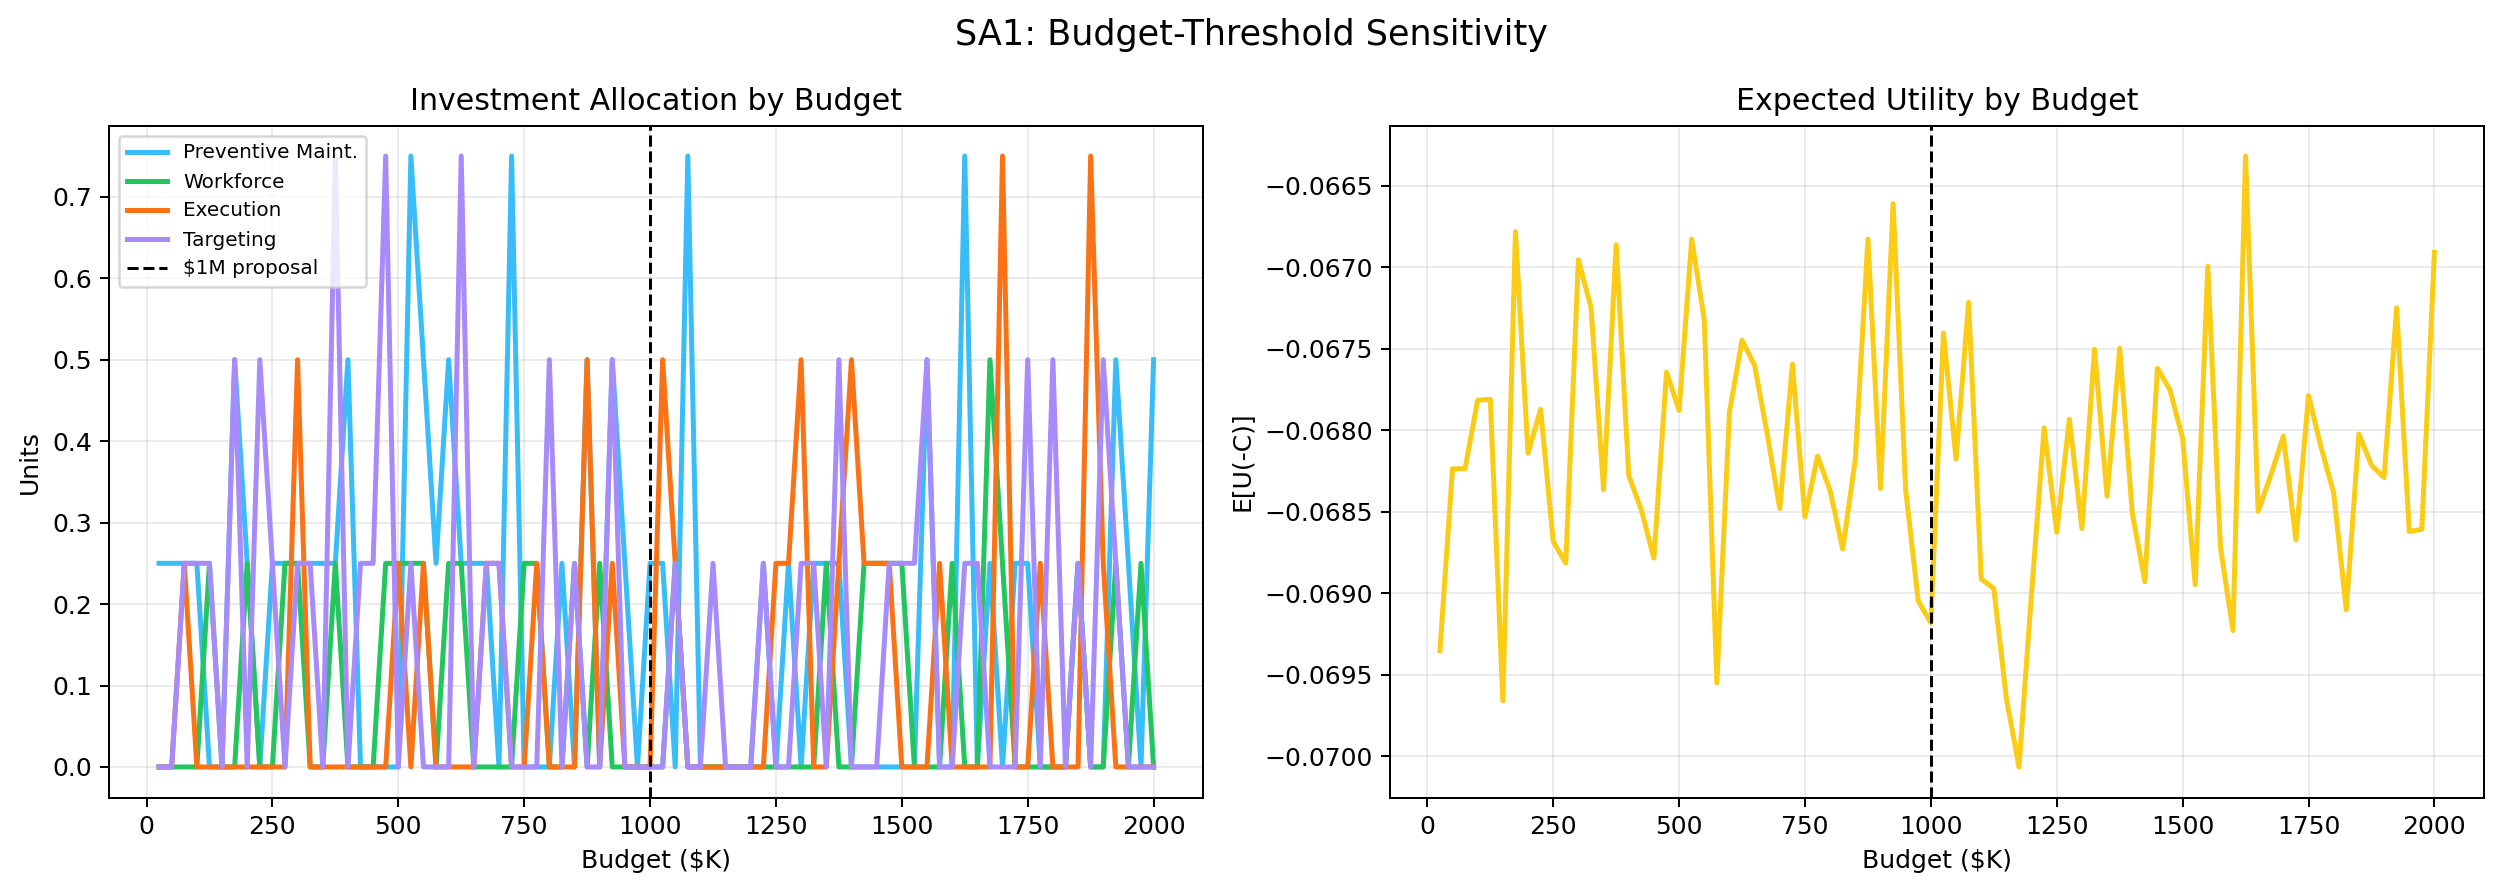
\includegraphics[width=\columnwidth]{figures/sa1_budget_sweep.png}
  \caption{Budget-threshold sensitivity analysis (SA1). Left: investment
    allocation by budget level; the optimizer places 100\% into
    Preventive Maintenance ($I_1$, blue) across the entire
    \$0--\$2M sweep. No second lever clears the entry threshold.
    Right: expected utility $E[U(-C)]$ as a function of budget,
    increasing monotonically. The dashed white line marks the
    \$1M board proposal. Seeded MC, 1{,}500 runs per point.}
  \label{fig:sa1}
\end{figure}

\subsection{Maintenance Cap: Investment Reallocation under Constraint}

\paragraph{Motivation.}
A second scenario asks what the optimizer does if the amount that
can be invested in preventive maintenance is administratively or
contractually capped---for example, if crew capacity limits
$I_1$ to \$300K (3 units) regardless of the total budget.
This analysis reveals how the model reallocates the remaining
budget across the other three levers when the dominant lever
is restricted.

\paragraph{Results.}
Table~\ref{tab:sa2-cap} reports the unconstrained and
maintenance-capped outcomes at the \$550K current-scenario budget
(5.5 units) for three cap levels: \$550K (unconstrained), \$300K,
and \$150K.

\begin{table}[H]
\centering
\caption{Maintenance-cap sensitivity (SA2). Budget fixed at \$550K
(5.5 units). All analyses seeded, 1{,}500 MC runs.}
\label{tab:sa2-cap}
\begin{tabular}{lcccccc}
\toprule
\textbf{Cap on $I_1$} & \boldmath$I_1$ & \boldmath$I_2$ &
  \boldmath$I_3$ & \boldmath$I_4$ &
  \textbf{$E[\lambda]$} & \textbf{$E[U]$} \\
\midrule
None (5.5 u)   & 5.50 & 0.00 & 0.00 & 0.00 & 4.37 & $-$0.041 \\
3.0 u (\$300K) & 3.00 & 0.00 & 0.00 & 2.50 & 4.89 & $-$0.047 \\
1.5 u (\$150K) & 1.50 & 0.25 & 0.00 & 3.75 & 5.36 & $-$0.052 \\
\bottomrule
\end{tabular}
\end{table}

When $I_1$ is capped at \$300K, the optimizer redirects the remaining
\$250K entirely to Risk-Based Targeting ($I_4$), which has the highest
effectiveness coefficient for blockage among the remaining levers
($\alpha_{B,I_4} = 0.028$). This is the model's rational response to
a binding maintenance constraint: it channels resources toward the
next-best blockage-mitigation lever. The expected annual spill rate
increases from 4.37 to 4.89 spills per year---a penalty of
0.52 additional expected spills per year, or approximately 12\% more
exposure than the unconstrained case---and expected utility falls from
$-0.041$ to $-0.047$.

At the tighter \$150K cap, the optimizer allocates the remaining
\$400K primarily to Risk-Based Targeting with a small residual to
Workforce Capacity ($I_2$), which contributes modestly to
blockage reduction via improved response effectiveness. Expected
annual spills rise to 5.36, and expected utility falls to $-0.052$.
Workforce Capacity and Execution Quality ($I_3$) enter only when
the two highest-return levers ($I_1$ and $I_4$) are exhausted,
consistent with their lower effectiveness coefficients for the
dominant blockage mode.

\begin{figure}[H]
  \centering
  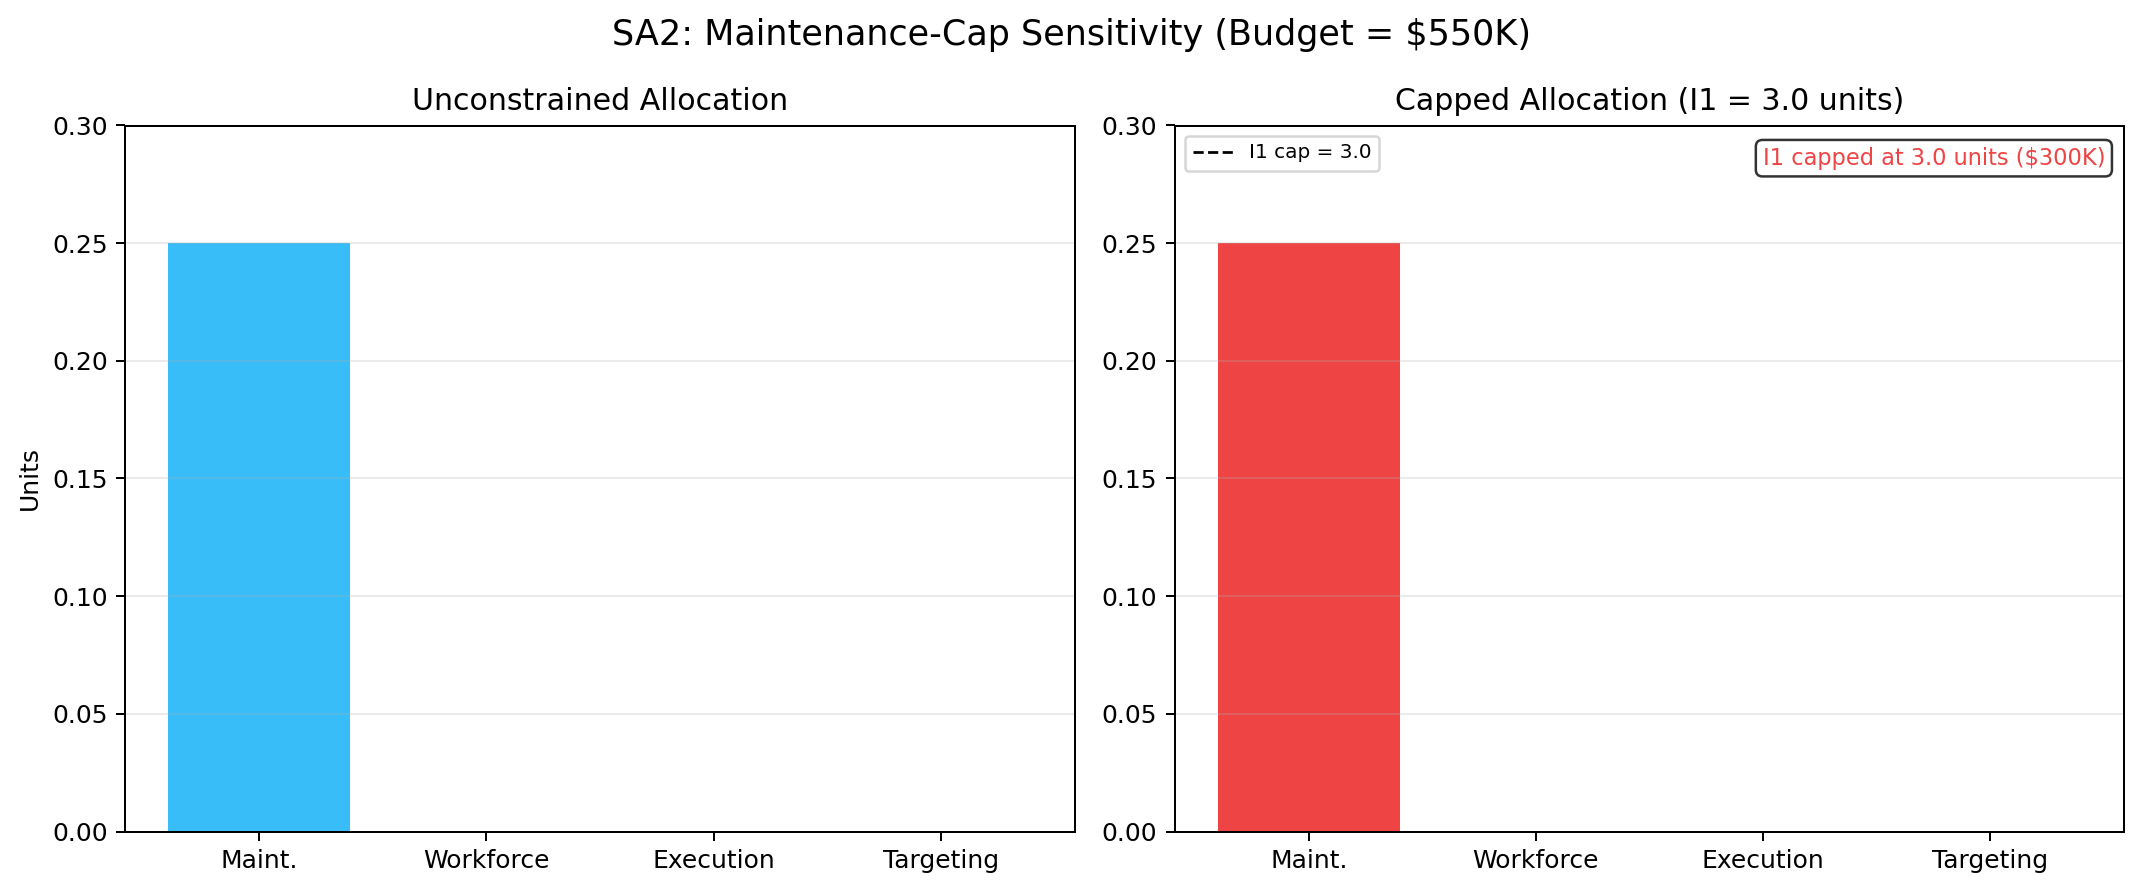
\includegraphics[width=\columnwidth]{figures/sa2_cap_comparison.png}
  \caption{Maintenance-cap sensitivity (SA2). Left: unconstrained
    optimal allocation at \$550K budget (all $I_1$). Right:
    allocation when $I_1$ is capped at \$300K (3 units); remaining
    \$250K redirected to Risk-Based Targeting ($I_4$, orange).
    Red bar indicates the constrained lever.}
  \label{fig:sa2}
\end{figure}

These results have a direct operational interpretation: even a
moderate restriction on preventive maintenance investment forces the
model to substitute toward targeting-based interventions, but the
substitution is imperfect. No combination of workforce, execution, or
targeting investments fully compensates for reduced maintenance,
because those levers primarily act on lower-frequency failure
modes. The blockage-reduction gap created by the maintenance cap
cannot be closed by reallocating to other levers alone; it requires
either lifting the cap or accepting higher expected spill frequency.

\subsection{Tornado Diagram: Cost Sensitivity to Extreme Assumptions}

\paragraph{Motivation.}
The cost model depends on three uncertain inputs that have been
estimated from historical data or calibrated priors: (1) the
per-spill volume distribution, (2) the failure rate $\lambda$, and
(3) the risk-tolerance parameter $\rho$. The tornado analysis
evaluates how expected annual cost and expected utility respond when
each of these inputs is moved individually from its minimum to its
maximum plausible extreme, with all other inputs held at their
base-scenario values. This identifies which uncertainties drive
the most output variation and deserve the most model-improvement
attention.

\paragraph{Parameter ranges.}
\begin{itemize}[noitemsep]
  \item \textbf{Spill volume (min $\to$ max):} Each spill is assigned
    the minimum possible volume for its severity category (category
    floors: 50 gal for Cat.~1, 1{,}001 gal for Cat.~2, 50 gal for
    Cat.~3, 1 gal for Cat.~4) or the maximum possible volume (category
    ceilings: 145{,}000 gal for Cat.~1, 50{,}000 gal for Cat.~2,
    1{,}000 gal for Cat.~3, 49 gal for Cat.~4), replacing the
    historical-bootstrap sampling.
  \item \textbf{Failure rate $\lambda$ ($\times 0.5 \to \times 2$):}
    All per-mode failure rates are scaled by a common factor of 0.5
    (optimistic system performance) or 2.0 (pessimistic), representing
    a $\pm 50$\% uncertainty band around the historical $\lambda_0$
    estimate.
  \item \textbf{Risk tolerance $\rho$ ($\times 0.1 \to \times 10$):}
    The utility parameter is shifted from \$1M (highly risk-averse) to
    \$100M (near-risk-neutral), capturing the full range of plausible
    board risk preferences.
\end{itemize}

\paragraph{Results.}
Figure~\ref{fig:sa3} and Table~\ref{tab:tornado} summarize the
tornado results relative to the base expected annual cost of
approximately \$605K under the optimized allocation. The figure
shows cost deviations in the left panel and expected-utility
deviations in the right panel, so the effect of changing
risk tolerance $\rho$ is visible even though raw cost is unchanged.

\begin{table}[H]
\centering
\caption{Tornado diagram summary (SA3). Base expected annual cost
  $\approx$ \$605K (optimized allocation, seeded MC, 4{,}000 runs).
  Swing $=$ max $-$ min expected cost.}
\label{tab:tornado}
\begin{tabular}{lcccr}
\toprule
\textbf{Variable} & \textbf{Low extreme} & \textbf{$E[\text{cost}]$ low}
  & \textbf{$E[\text{cost}]$ high} & \textbf{Swing} \\
\midrule
Spill volume (min $\to$ max) & Cat.\ floors
  & $\sim$\$448K & $\sim$\$1.62M & $\sim$\$1.17M \\
Failure rate $\lambda$ ($\times 0.5 \to \times 2$) & $\lambda \times 0.5$
  & $\sim$\$301K & $\sim$\$1.21M & $\sim$\$0.91M \\
Risk tolerance $\rho$ ($\times 0.1 \to \times 10$) & $\rho = \$1$M
  & \multicolumn{2}{c}{(utility scale only; raw cost unchanged)} & --- \\
\bottomrule
\end{tabular}
\end{table}

\textbf{Spill volume is overwhelmingly the dominant cost driver.}
When all spills occur at minimum volume (category floors), expected
annual cost falls to approximately \$448K---a reduction of
about \$157K from the \$605K base. When all spills occur at maximum
volume (category ceilings), expected annual cost rises to approximately
\$1.62M, an increase of about \$1.01M above base. The total swing is
therefore roughly \$1.17M, confirming that the upper tail of the
volume distribution still dominates the expected-cost calculation.
This has two implications
for CAWD: (i) the historical record contains genuine tail events
(the 2017 Hatton Canyon pipe failure at 145{,}000 gallons and the
2023 pipe failures totaling over 93{,}000 gallons) that are
appropriately classified as high-impact outliers, and (ii) any
intervention that reduces spill volumes---such as faster response
times or real-time monitoring that enables early shutoff---carries
a cost benefit disproportionate to its effect on spill frequency.

\textbf{Failure rate uncertainty is the second-largest driver.}
Scaling all $\lambda$ values by 0.5 (reflecting an optimistic
scenario in which infrastructure condition improves markedly)
reduces expected annual cost to approximately \$301K. Scaling by 2.0
(reflecting a pessimistic scenario of accelerated aging or
under-investment) raises it to approximately \$1.21M. The total
swing of approximately \$0.91M reflects the fact that expected cost
is proportional to expected spill frequency, which is linear in
$\lambda$ through the Poisson model. This confirms that the rate
estimates $\lambda_0$---drawn from 25.25 years of CAWD history after
removing the 2020 zero-spill year---are the dominant structural
input: a systematic over- or undercount of historical failures would
propagate directly into cost estimates with near-linear scaling.

\textbf{Risk tolerance $\rho$ affects utility but not raw cost.}
Because $\rho$ enters only through the exponential utility function
$U(-C) = 1 - e^{C/\rho}$ and not through the cost simulation
itself, varying $\rho$ does not change expected annual cost. At
$\rho = \$1$M (very risk-averse, $\rho \times 0.1$), the utility
function is highly concave and severely penalizes tail outcomes:
$E[U]$ falls from approximately $-0.063$ to $-0.948$, and the
optimizer under this setting would
be expected to shift even more of the budget toward prevention. At
$\rho = \$100$M (near-risk-neutral, $\rho \times 10$), $E[U]$
increases to approximately $-0.006$, approaching $-E[C]/\rho$, and
the objective reduces approximately to expected-cost minimization.
The calibrated value $\rho = \$10$M
(board-elicited, $1/\gamma \approx \$11$M) lies between these
extremes and is consistent with the board placing material weight
on tail outcomes without being dominated by worst-case scenarios.
The insensitivity of the cost metrics to $\rho$ confirms that the
raw cost projections in Table~\ref{tab:mc-results} are not artifacts
of the utility calibration.

\begin{figure}[H]
  \centering
  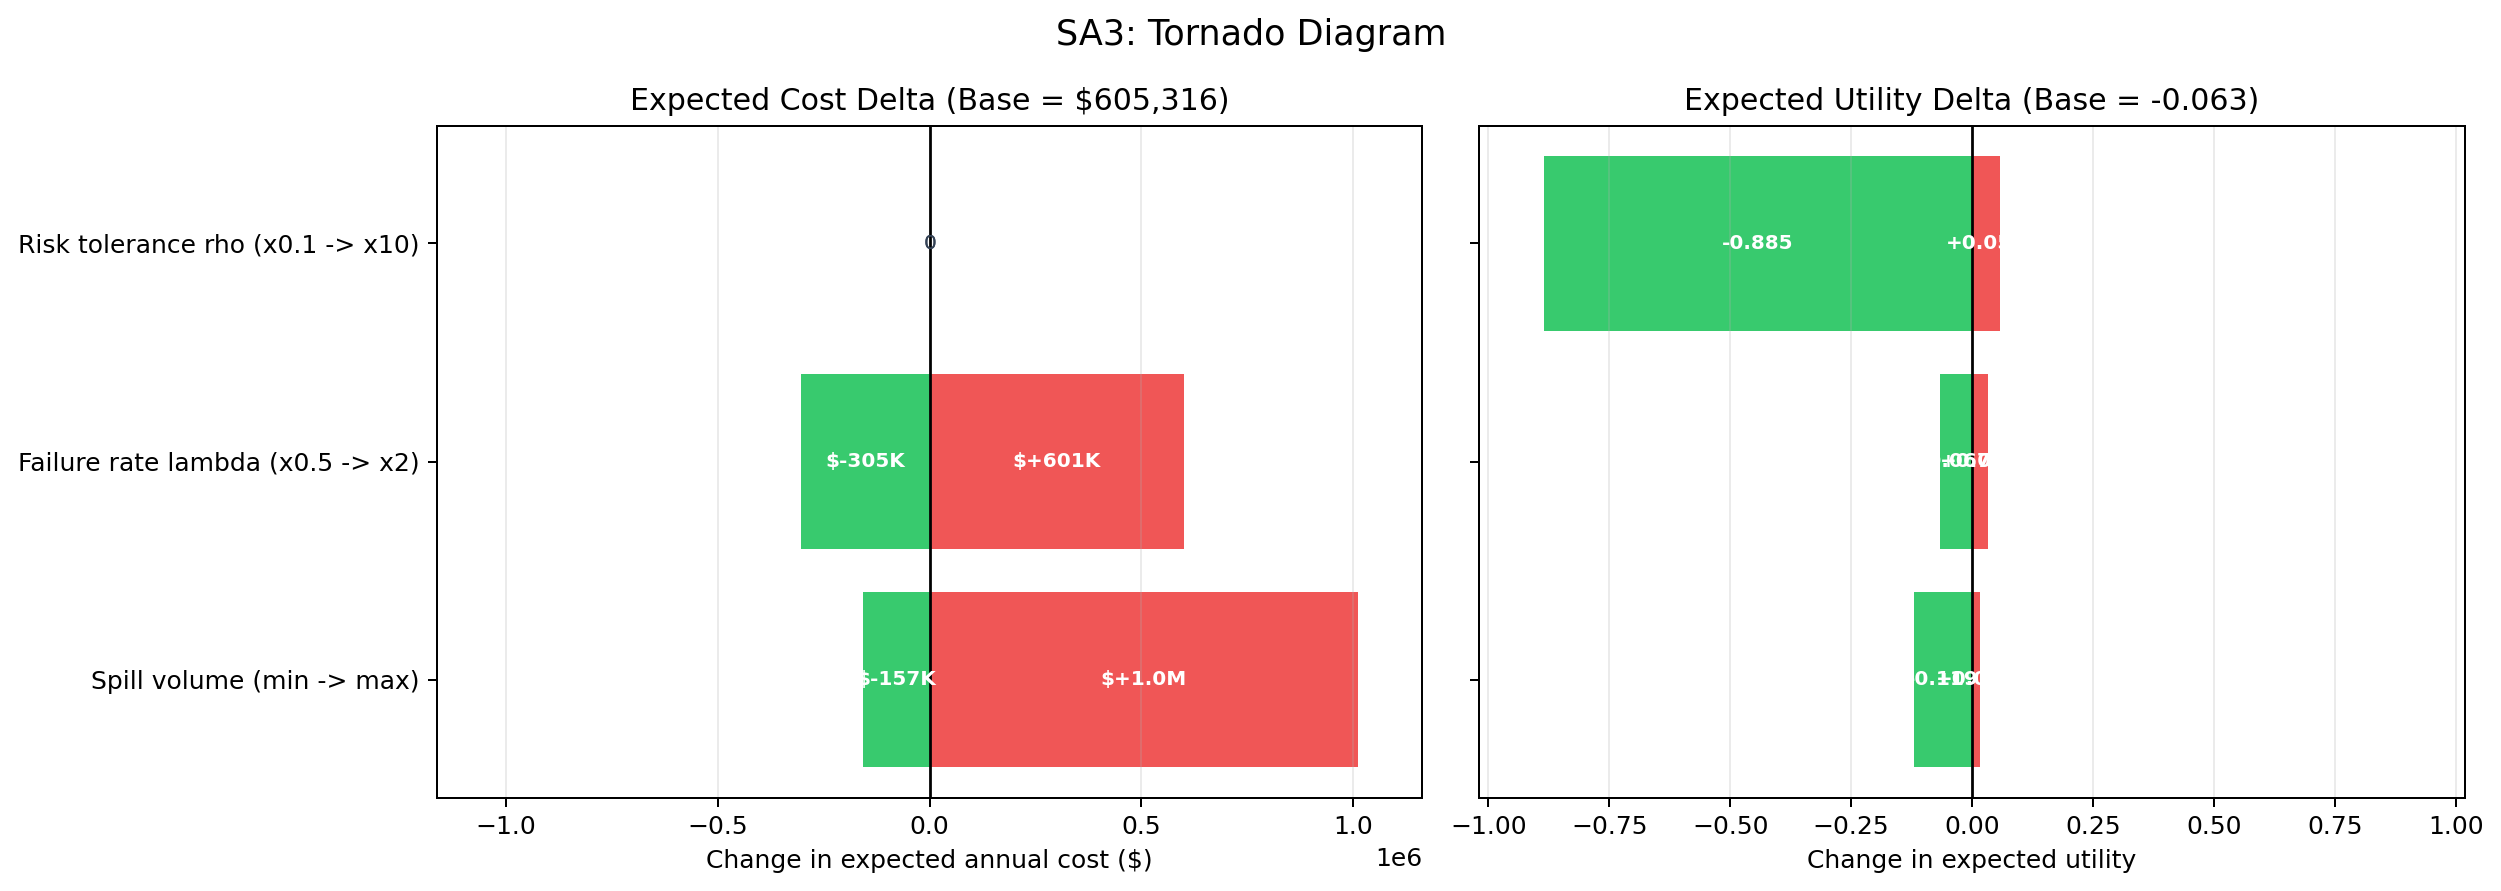
\includegraphics[width=\columnwidth]{figures/sa3_tornado.png}
  \caption{Tornado diagram (SA3). Left: deviation of expected annual
    cost from the base scenario (\$605K) when one input is set to
    its low (green, cost-reducing) or high (red, cost-increasing)
    extreme. Right: deviation of expected utility from the base
    scenario under the same perturbations. Spill volume dominates the
    cost swing, failure-rate uncertainty is second, and risk
    tolerance $\rho$ appears only in the utility panel because it
    changes preferences rather than raw spill cost. Values are
    printed inside each bar.}
  \label{fig:sa3}
\end{figure}

\paragraph{Summary of sensitivity findings.}
The three analyses collectively characterize the decision space in
which CAWD operates. The budget-threshold analysis establishes that
the all-maintenance recommendation is structurally robust across a
wide budget range---it is not an artifact of the \$1M constraint.
The maintenance-cap analysis shows that if operational capacity
limits $I_1$, the model's rational fallback is Risk-Based Targeting,
at a cost of roughly 0.5 additional expected spills per year per
\$250K of maintenance withheld. The tornado analysis establishes that
volume uncertainty---particularly the possibility of another
tail event like 2017 or 2023---is the dominant source of cost
variance, with failure rate uncertainty a distant second. Together,
these findings suggest that the highest-value risk-reduction actions
for CAWD are (i) sustaining preventive maintenance at full budgeted
levels, (ii) investing in response-time improvements that limit
spill volumes once a failure begins, and (iii) improving the
historical failure-rate record by reducing the share of
unclassified-cause (``U'') spill events.

%============================================================
\section{Discussion}
\subsection{Limitations}
 
Several limitations of the present study should be noted when
interpreting the results and considering the framework's
applicability.
\textbf{Sparse historical data for three failure modes.} Pump
failure, hydraulic overload, and operational failure rates are
assigned using operational priors rather than estimated from
historical CAWD records, because no labeled events of these types
appear in the 26-year spill tracking dataset. While the priors
are grounded in engineering judgment and industry benchmarks,
they introduce unquantified uncertainty into the cost distribution.
In particular, the hydraulic overload prior rate of 0.20 spills
per 100 miles per year may understate true risk if the absence
of labeled events reflects data-coding practices rather than
genuine rarity. The sensitivity of the optimization result to
these prior values is not formally characterized in this study.

\textbf{Single-utility calibration.} All model parameters ---
baseline rates, severity distributions, volume arrays, and cost
structures --- are calibrated exclusively to CAWD. The framework
is designed to be transferable to other utilities, but the
specific numerical outputs (the optimal allocation, the baseline
cost distribution, the tail-risk probabilities) reflect CAWD's
particular infrastructure composition, climate, and regulatory
environment. Applying the framework to a different utility would
require full recalibration of all parameters from that utility's
historical records.

\textbf{Pipe blockage model performance.} The root blockage
logistic regression model achieves an AUC of 0.589, which
provides useful rank-ordering of pipes by relative risk but
falls short of strong discriminative performance. Root intrusion
is spatially distributed across the system with no dominant
geographic cluster, limiting the feature signal available to
the model. The CRI rankings should therefore be interpreted as
relative risk indicators rather than absolute probability
estimates, and field inspection should be used to validate
high-CRI segments before committing maintenance resources.

\subsection{Future Work}
 
Several directions would extend and strengthen the framework
developed in this study.
 
\textbf{Geographical risk decomposition.} The current framework
aggregates spill risk at the system level, treating the 77.57-mile
collection network as a single unit for rate estimation and
optimization. A natural extension would decompose the analysis
by drainage basin or geographic subarea, identifying which
areas of the CAWD service territory contribute disproportionately
to the total risk of the system. This spatial disaggregation would allow
maintenance resources to be targeted not only at the highest-CRI
individual pipes but at the highest-risk spatial clusters,
enabling more operationally actionable guidance for field crews.
The CAWD spill tracking record includes location information that
would support this analysis without requiring additional data
collection.
 
\textbf{Pipe remaining useful life estimation.} The logistic
regression model developed in this study predicts blockage
probability as a static function of current pipe characteristics.
A more powerful extension would model pipe deterioration as a
dynamic process, estimating the remaining useful life of each
segment and identifying when pipes should be replaced rather
than cleaned. Survival analysis methods --- including
semi-Markov models of the type used in infrastructure asset
management literature \citep{kleiner2001} --- would allow the
framework to generate a forward-looking replacement schedule
rather than only a current-state maintenance priority list.
This would directly support CAWD's multi-year Capital Improvement
Program planning by providing data-driven input to the pipe
replacement queue.
 
\textbf{Validation on larger sewer systems.} The present study
is calibrated to a small utility serving approximately 11{,}000
residents across 81 miles of infrastructure. It would be valuable
to evaluate whether the framework produces reliable optimization
recommendations when applied to a larger sewer system ---
for example, a mid-sized city utility with several hundred miles
of pipe and a more diverse failure mode distribution. Larger
systems would provide more statistical power for failure-mode
rate estimation, reducing dependence on operational priors, and
would test whether the corner solution result is specific to
CAWD's particular failure-mode structure or is a more general
property of systems where one failure mode strongly dominates.

\textbf{Dynamic investment optimization.} The current framework
treats the O\&M budget allocation as a single-period decision.
A multi-period extension would allow the optimizer to recommend
investment sequences that account for the fact that sustained
preventive maintenance investment changes the baseline failure
rate over time, potentially making other investment levers
relatively more attractive in later periods as blockage risk
declines.

% ============================================================
\section{Conclusions}
% ============================================================

% TODO: Summarize:
% - PRA framework
% - optimization contribution
% - risk-aversion contribution
% - operational applicability
% - infrastructure risk-management implications

% ============================================================
\appendix
% ============================================================

%\section{Mathematical Derivations}

% TODO: Include:
% - KKT derivations
% - expected utility derivations


\section{Monte Carlo Algorithm}

\begin{enumerate}[leftmargin=*]

\item Input:
\begin{itemize}
    \item Baseline failure rates $\lambda_k^0$
    \item Effectiveness matrix $\alpha_{ki}$
    \item Category probabilities $q_{kc}$
    \item Spill volume distributions
    \item Investment allocation $I$
\end{itemize}

\item Compute investment-adjusted failure rates

\[
\lambda_k(I)
=
\lambda_k^0
\exp
\left(
-\sum_i \alpha_{ki} I_i
\right).
\]

\item For each simulated year:

\begin{enumerate}

\item For each failure mode $k$, sample

\[
N_k \sim \text{Poisson}(\lambda_k(I)).
\]

\item For each spill event:

\begin{enumerate}

\item Sample severity category from $q_{kc}$.

\item Sample spill volume from the historical or fitted volume distribution.

\item Compute spill consequence cost.

\end{enumerate}

\item Aggregate spill-event costs to obtain

\[
C(I,\omega)
=
\sum_j C_j.
\]

\end{enumerate}

\item Repeat for 50{,}000 simulated years.

\item Compute expected annual cost, percentile risk measures,
probability of annual cost exceeding \$1M, and expected utility.

\end{enumerate}

\section{Supplementary Tables}

Tables~\ref{tab:pipe-char} and~\ref{tab:pipe-maint} present a representative
sample of the CAWD Integrated Dataset used in this study. Both tables draw
from the same spreadsheet, split here solely due to page width constraints.
Table~\ref{tab:pipe-char} shows pipe identity attributes (asset identifier,
diameter, length, material, installation year, and flow basin) and
Table~\ref{tab:pipe-maint} shows the corresponding inspection and maintenance
history for the same pipe segments, including last cleaning date, last recorded
spill date, total cleaning count, and the most recent grease and roots condition
scores from cleaning observations. Note that Last Cleaning Date appears in the
dataset but was excluded from model estimation. The full integrated dataset
covers 1,864 pipe segments and is described in Section~4.1.

\begin{table*}[h]
\centering
\caption{CAWD Integrated Data: Pipe Characteristics}
\label{tab:pipe-char}
\begin{tabular}{p{2cm} p{1.5cm} p{1.5cm} p{2cm} p{1cm} p{3.5cm}}
\toprule
\textbf{Asset ID} & \textbf{Diameter (in)} & \textbf{Length (ft)} & \textbf{Pipe Material} & \textbf{Install Year} & \textbf{Flow Basin}\\
\midrule
O816-O904 & 6  & 193.5 & VCP  & 1973 & Hatton Basin \\
N661-O692 & 6  & 220.4 & VCP  & 1908 & Midtown Basin \\
N609-N610 & 8  & 374.6 & PVC  & 1924 & Beach Basin \\
O728-O735 & 6  & 304.7 & VCP  & 1961 & Paradise Park Basin \\
Q806-Q807 & 10 & 472.6 & HDPE & 2019 & Hatton Basin \\
\bottomrule
\end{tabular}
\end{table*}

\begin{table*}[h]
\centering
\caption{CAWD Integrated Data: Inspection \& Maintenance History}
\label{tab:pipe-maint}
\begin{tabular}{p{2cm} p{2cm} p{2cm} p{2.5cm} p{1.8cm} p{2cm}}
\toprule
\textbf{Asset ID} & \textbf{Last Cleaning Date} & \textbf{Last Spill Date} & \textbf{Total Cleaning} & \textbf{Last Grease Rating} & \textbf{Last Root Rating}\\
\midrule
O816-O904 & 2023-08-18 & 2014-06-20 & 13 & 1 & 1 \\
N661-O692 & 2024-02-22 & 2014-09-16 & 16 & 1 & 1 \\
N609-N610 & 2024-01-26 & 2014-10-24 & 22 & 1 & 1 \\
O728-O735 & 2023-08-31 & 2014-10-29 & 17 & 1 & 1 \\
Q806-Q807 & 2023-10-18 & 2020-12-07 & 13 & 1 & 1 \\
\bottomrule
\end{tabular}
\end{table*}


% TODO: Add spill reclassification tables, sensitivity tables,
% and scenario comparison tables
\newpage
\bibliographystyle{apalike}
\bibliography{references}

\end{document}